%----------------------------------------------------------------
%
%  File    :  survey.tex
%
%  Author  :  Keith Andrews, ISDS, TU Graz, Austria
%
%  Created :  24 Mar 2010
%
%  Changed :  22 Jan 2021
%
%----------------------------------------------------------------


\documentclass[11pt,onecolumn,twoside]{report}

\usepackage[
  a4paper,
  twoside,
  top=5mm,                % top margin
  bottom=7mm,             % bottom margin
  inner=20mm,             % inner margin (next to binding)
  outer=20mm,             % outer margin (opposite binding)
  bindingoffset=10mm,     % on binding side
  includeheadfoot,        % include head(er) and foot(er)
  headheight=10mm,        % height of header
  headsep=15mm,           % sep between header and text body
  footskip=15mm,          % sep between body and baseline of footer
  footnotesep = 10mm plus 2mm minus 0mm  % bottom of body to top of footnote
]{geometry}
% A4 paper is w=210m, h=297mm


\newcommand{\thistitle}{Checking Web Accessibility}  % title
% \newcommand{\thissubject}{Guidelines for Writing a Survey Paper in Computer Science}  % subject
\newcommand{\thissubject}{}  % leave empty for no subject
\newcommand{\thisauthor}{Ožbej Golob, Alexander Thien, Olli-Pekka Riikola, Robin Karlsson}          % author
% \newcommand{\thisauthor}{Keith Andrews, Tom Black, and Harry White}      % multiple authors
\newcommand{\thiskeywords}{web accessibility, screen readers, text-only browsers, accessibilty audit tools}   % keywords

\newcommand{\thisdate}{12 Dec 2022}  % date of this version
\newcommand{\thisyear}{2022}         % year of this version




\newcommand{\fullh}{24cm}         % height of figures for 1 per page
\newcommand{\halfh}{9.5cm}        % height of figures for 2 per page
\newcommand{\thirdh}{6cm}         % height of figures for 3 per page


\setlength{\parindent}{1em}       % less indentation
\setlength{\parskip}{5pt plus 1pt minus 1pt}  % space before a paragraph


% \tolerance is set by LaTeX to 200
% \sloppy sets \tolerance = 9999
% which allows LaTeX more tolerance in adding word spacing

% \sloppy
% \fussy
% \tolerance = 1000

\tolerance=400 
% makes some lines with lots of white space, but      
% tends to prevent words from sticking out in the margin



\setcounter{tocdepth}{3}        % lowest section level entered in ToC
\setcounter{secnumdepth}{3}     % lowest section level still numbered




\usepackage[T1]{fontenc}        % 8-bit output chars (must be before inputenx)
\usepackage[utf8]{inputenx}     % input char encoding

\usepackage[english,austrian,british]{babel}

\usepackage{newtxtext}          % newer times fonts
\usepackage{newtxmath}

\usepackage{relsize}            % relative font sizes \smaller \larger
\usepackage{float}              % H for float placement
\usepackage{setspace}           % line spacing

\usepackage{textcomp}           % symbols such as \texttimes and \texteuro
\usepackage{latexsym}
\usepackage{fontawesome}        % fontawesome symbols

\usepackage{siunitx}            % prettier number formatting
\sisetup{%
  group-separator={,},
}
\usepackage[super]{nth}         % 1st, 2nd, 3rd, etc.

\usepackage{xspace}
\usepackage{xstring}            % string manipulation macros
\usepackage{xparse}             % commands with optional arguments
\usepackage{etoolbox}           % for \newrobustcmd
\usepackage{makecmds}           % for \makecommand
\usepackage{calc}               % for math calculations

\usepackage[svgnames,table,xcdraw]{xcolor}
\definecolor{darkgreen}{rgb}{0.0,0.2,0.0}
\definecolor{darkblue}{rgb}{0.0,0.0,0.2}
\definecolor{darkred}{rgb}{0.2,0.0,0.0}
\definecolor{verylightgrey}{gray}{0.95}
\definecolor{lightgrey}{gray}{0.9}
\definecolor{grey}{gray}{0.7}
\definecolor{black}{gray}{0.0}

\definecolor{tableheadercolour}{gray}{0.8}
\definecolor{tablerowcolour}{gray}{0.93}



\usepackage{longtable}
\usepackage{multirow}
\usepackage{tabularx}

% Define some new column types for tables:
% like X but flushleft (= raggedright) rather than justified
\newcolumntype{Y}{>{\raggedright\arraybackslash}X}
% a p column but flushleft (= raggedright) rather than justified
\newcolumntype{L}[1]{>{\raggedright\arraybackslash}p{#1}}
% a p column but flushright (= raggedleft) rather than justified
\newcolumntype{R}[1]{>{\raggedleft\arraybackslash}p{#1}}


\usepackage{booktabs}           % nicer tables

\newcommand{\tablestretch}
{\renewcommand{\arraystretch}{1.20}}  % spacing between table rows




\usepackage{verbdef}            % define robust verb strings
\usepackage{verbatim}
\usepackage{comment}



% better lists
\usepackage{enumitem}

\setlist{
  topsep=0pt,
  partopsep=0pt,
  parsep=0.6ex,
  itemsep=1.2ex,
  left=\parindent .. 2\parindent,    % bullet .. start ot text
}

\setlist[description]{
  style=sameline,
}




\usepackage{listings}                 % for listings of source code

\makeatletter
\newlength{\numwidth}%
\setlength{\numwidth}{\widthof{\normalfont{\lst@numberstyle{99}}}}% Up to 2-digit (99) line numbers
\def\lst@PlaceNumber{%
  \makebox[\numwidth+1em][l]{%
    \makebox[\numwidth][r]{\normalfont\lst@numberstyle{\thelstnumber}}%
  }%
}
\makeatother

% lstset strategy: define defaults here for
% all non-floating (displayed) listings
% floated listings override these settings later

\lstset{                              % set parameters for listings
  floatplacement=tp,                  % default float placement
  numberbychapter,
  inputencoding=utf8,
  language=,                          % empty = plain text
  basicstyle=\small\ttfamily,
  tabsize=2,
  xleftmargin=2\parindent,
  xrightmargin=2\parindent,
  frame=none,
  framexleftmargin=0mm,
  rulesepcolor=\color{verylightgrey},
  numbers=none,
  numberstyle=\scriptsize,
  numbersep=2ex,
  breaklines,
  showtabs=false,
  showspaces=false,
  showstringspaces=false,
  keywordstyle=\color{black},
  commentstyle=\color{SteelBlue},
  identifierstyle=,
  stringstyle=,
  captionpos=b,
  abovecaptionskip=\abovecaptionskip,
  belowcaptionskip=\belowcaptionskip,
  extendedchars=true,           % listings usually only support 7-bit ascii chars
  literate=%                    % map some one-byte utf8 chars for use in listings
%    { }{{~}}1                   % non-breaking space
    {©}{{\textcopyright}}1
    {€}{{\texteuro}}1
    {Ö}{{\"O}}1
    {Ä}{{\"A}}1
    {Ü}{{\"U}}1
    {ß}{{\ss}}1
    {ö}{{\"o}}1
    {ä}{{\"a}}1
    {ü}{{\"u}}1,
}


\lstdefinelanguage{biblatex}   % based on biblatex v 2.7a from 2013-07-14
{
  keywords={%
    @article,@book,@mvbook,@inbook,@bookinbook,@suppbook,%
    @booklet,@collection,@mvcollection,@incollection,@suppcollection,%
    @manual,@misc,@online,@patent,@periodical,@suppperiodical,%
    @proceedings,@mvproceedings,@inproceedings,@reference,@mvreference,%
    @inreference,@report,@set,@thesis,@unpublished,@xdata,%
    @conference,@electronic,@mastersthesis,@phdthesis,@techreport,@www,%
    @artwork,@audio,@bibnote,@commentary,@image,@jurisdiction,@legislation,%
    @legal,@letter,@movie,@music,@performance,@review,@software,%
    @standard,@video%
  },
  sensitive=false,
  comment=[l][\itshape]{@comment},
  morecomment=[l]{\%},
}

\lstdefinelanguage{CSS}
{
  alsoletter={-},
  morekeywords={%
  color,background,background-color,margin,padding,font,
  font-family,weight,%
  display,position,top,left,right,bottom,list,%
  style,border,size,white,space,min,width%
  },
  sensitive=false,
  morecomment=[l]{//},
  morecomment=[s]{/*}{*/},
  morestring=[b]",
}





\usepackage[compact,nobottomtitles,pagestyles,explicit]{titlesec}
% when using explicit, must explicitly include #1 for titlename

% nobottomtitles
% move section headings close to page bottom to next page
\renewcommand{\bottomtitlespace}{2cm}

% \chaptermark sets the value of \chaptertitle for later
% \@chapapp is defined as \chaptername outside the appendix,
% and as \appendixname within the appendix.
\makeatletter
\titleformat{\chapter}
[display]                                            % shape
{\chaptermark{\thechapter~~#1}\sffamily\bfseries}    % format
{\huge\@chapapp\ \thechapter}                        % label
{4ex}                                                % sep
{\Huge#1}                                            % before-code
\makeatother

\titleformat{name=\chapter,numberless}
[block]                                              % shape
{\chaptermark{#1}\sffamily\bfseries}                 % format
{}                                                   % label
{0ex}                                                % sep
{\Huge#1}                                            % before-code

\titleformat{\section}
{\normalfont\Large\sffamily\bfseries}{\thesection}{0.8em}{#1}

\titleformat{\subsection}
{\normalfont\large\sffamily\bfseries}{\thesubsection}{0.8em}{#1}

\titleformat{\subsubsection}
{\normalfont\normalsize\sffamily\bfseries}{\thesubsubsection}{0.8em}{#1}

\titleformat{\paragraph}[runin]
{\normalfont\normalsize\sffamily\bfseries}{\theparagraph}{0.8em}{#1}

\titleformat{\subparagraph}[runin]
{\normalfont\normalsize\sffamily\bfseries}{\thesubparagraph}{0.8em}{#1}


% vertical spacing before and after section titles
\titlespacing*{\section}
{0pt}{3.5ex plus 0.5ex minus 0.5ex}{0ex plus 0ex minus 0.2ex}

\titlespacing*{\subsection}
{0pt}{2.5ex plus 0.5ex minus 0.5ex}{0ex plus 0ex minus 0.2ex}

\titlespacing*{\subsubsection}
{0pt}{2ex plus 0.5ex minus 0.5ex}{0ex plus 0ex minus 0.2ex}


% define page headings how I want them

\newpagestyle{main}[\small]{
% \addtolength\headheight{6.7pt}
% \headrule
\sethead%
[{\parbox[t]{0.3\textwidth}%                    % even left
  {\sffamily\thepage}}]
[]%                                             % even centre
[{\parbox[t]{0.6\textwidth}%                    % even right
  {\raggedleft\sffamily\chaptertitle}}]
{{\parbox[t]{0.6\textwidth}%                    % odd left
  {\sffamily\sectiontitle}}}%
{}%                                             % odd centre
{{\parbox[t]{0.3\textwidth}%                    % odd right
  {\raggedleft\sffamily\thepage}}}
}




\usepackage{titletoc}

% \contentsmargin{2.55em}

\titlecontents{chapter}%
[1.5em]%                         % left indent to entry text
{\addvspace{1em}\bfseries}%      % above-code per entry
{\contentslabel{1.5em}}%         % format for numbered entry
{\hspace*{-1.5em}}%              % format for unnumbered entry
{\hfill\contentspage}%           % [no dots] and page num per entry


% Note: \dottedcontents is short form of \titlecontents

\dottedcontents{section}%
[3.8em]%                         % left indent to entry text = 1.5 + 2.3
{}%                              % above-code per entry
{2.3em}%                         % label width
{1pc}%                           % space around the dots

\dottedcontents{subsection}%
[7.4em]%                         % left indent to entry text = 3.8 + 3.6
{}%                              % above-code per entry
{3.6em}%                         % label width
{1pc}%                           % space around the dots


\dottedcontents{figure}%         % LoF entries
[3.0em]%                         % left indent to entry text = 3.8 + 3.6
{}%                              % above-code per entry
{3.0em}%                         % label width
{1pc}%                           % space around the dots

\dottedcontents{table}%          % LoT entries
[3.0em]%                         % left indent to entry text = 3.8 + 3.6
{}%                              % above-code per entry
{3.0em}%                         % label width
{1pc}%                           % space around the dots



% List of Listings is unknown to titletoc, define here

% Add extra per-chapter space to LoL to mimic LoF and LoT
% (requires package etoolbox)
\makeatletter
\patchcmd{\@chapter}% <cmd>
  {\addtocontents}% <search>
  {\addtocontents{lol}{\protect\addvspace{10\p@}}% add per-chapter space
   \addtocontents}% <replace>
  {}{}% <success><failure>
\makeatother

% Configure LoL to mimic LoF and LoT
\contentsuse{lstlisting}{lol}

\titlecontents{lstlisting}%
[3.0em]%                              % left indent
{\addvspace{1.5mm}}%                  % above-code per entry
{\contentslabel{3.0em}}%              % format for numbered entry
{\hspace*{-3.0em}}%                   % format for unnumbered entry
{\titlerule*[1pc]{.} \contentspage}%  % dots and page num per entry
[]%                                   % below-code per entry

\renewcommand{\lstlistlistingname}{List of Listings}






% sensible settings for floats

\setlength{\textfloatsep}{9mm plus 2mm minus 2mm}
\setlength{\floatsep}{9mm plus 2mm minus 2mm}
\setlength{\intextsep}{9mm plus 2mm minus 2mm}

\setlength{\dbltextfloatsep}{9mm plus 2mm minus 2mm}
\setlength{\dblfloatsep}{9mm plus 2mm minus 2mm}

\setlength{\abovecaptionskip}{4mm plus 2mm minus 1mm}
\setlength{\belowcaptionskip}{2mm plus 1mm minus 1mm}


% See http://www-rohan.sdsu.edu/~aty/bibliog/latex/floats.html
% See https://robjhyndman.com/hyndsight/latex-floats/

\setcounter{topnumber}{2}               % max num floats at top of page
\setcounter{dbltopnumber}{2}            % max num floats on 2col page
\setcounter{bottomnumber}{2}            % max num floats at bottom of page
\setcounter{totalnumber}{4}             % max num floats on a page

\renewcommand{\topfraction}{0.8}        % max fraction of floats at top
\renewcommand{\dbltopfraction}{0.9}     % max fraction of floats at top 2col
\renewcommand{\bottomfraction}{0.8}     % max fraction of floats at bottom
\renewcommand{\textfraction}{0.2}       % min fraction of text

% only for entirely float pages:
\renewcommand{\floatpagefraction}{0.7}      % min page fraction having floats
\renewcommand{\dblfloatpagefraction}{0.7}   % min 2col page fraction having floats


% \usepackage[section,above,below]{placeins}  % keep floats to their own section




% use caption and subfig (caption2 and subfigure are now obsolete)

\usepackage[
  position=bottom,
  margin=1cm,
  font=small,
  labelfont={bf,sf},
  format=plain,
  indention=5mm,
  aboveskip=4mm,
  belowskip=0mm,
]{caption,subfig}

\captionsetup[subfigure]{
  margin=0pt,
  parskip=0pt,
  indention=5mm,
  farskip=4mm,            % skip above subfig (assuming captions at bottom)
  captionskip=2mm,        % skip between subfig and subcaption
}




\usepackage[short]{datetime}   % load datetime *after* babel, requires fmtcount
% \newdateformat{britdate}{%
% \ordinaldate{\THEDAY} \,\monthname[\THEMONTH] \THEYEAR
% }
\newdateformat{unixdate}{%
\twodigit{\THEDAY}~\shortmonthname[\THEMONTH]~\THEYEAR
}



\usepackage[
  autostyle=true,          % adapt quote style to current language
  english=british,         % british english as default
  threshold=1,             % set block quotations >1 line in display mode
  maxlevel=4,              % max nesting level
]{csquotes}

\usepackage[
  indentfirst=false,
  vskip=0pt,               % by default would be \topsep + \partopsep.
]{quoting}

% tell csquotes to use quoting environment
% for \displayquote and \blockquote
\SetBlockEnvironment{quoting}

% if cite is issued by a csquote command
\renewcommand{\mkcitation}[1]{\space#1}

% I prefer double quotes as outer
\DeclareQuoteStyle{keithbritish}%  [variant]{style}
  {\textquotedblleft}%                      opening outer mark
  {\textquotedblright}%                     closing outer mark
  [0.05em]%
  {\textquoteleft}%                         opening inner mark
  {\textquoteright}%                        closing inner mark

\ExecuteQuoteOptions{style=keithbritish}





\usepackage[
  backend=biber,
%  style=ext-authoryear-comp,   % defined in biblatex-ext package
  style=ext-authoryear,        % defined in biblatex-ext package
  sorting=nyt,
  useprefix,                   % van and von are part of second name
  mergedate=false,             % only for authoryear style
  dashed=false,                % only for authoryear style
  abbreviate=false,
  maxcitenames=2,              % if > 2 authors,
  mincitenames=1,              % use first 1 then et al
  maxbibnames=99,              % if > 99 authors,
  minbibnames=6,               % use first 6 then et al
  uniquelist=minyear,
  uniquename=init,
  hyperref=true,
  backref=true,
  backrefstyle=two,
  sortlocale=en,
]{biblatex}



% set for csquotes, but \autocite only available
% after biblatex is loaded
\SetCiteCommand{\autocite}    % or maybe \parencite

% more space between entries in bib
\setlength\bibitemsep{1.5\itemsep}

% kandrews: replace round brackets with square brackets in citations
\DeclareOuterCiteDelims{parencite}{\bibopenbracket}{\bibclosebracket}
\DeclareInnerCiteDelims{textcite}{\bibopenbracket}{\bibclosebracket}

% kandrews: replace round brackets with square brackets in bibliography
% biblabeldate is a biblatex-ext feature
\DeclareFieldFormat{biblabeldate}{\mkbibbrackets{#1}}


% remove URL: from in front of URLs
\DeclareFieldFormat{url}{\url{#1}}
\DeclareFieldFormat{doi}{\doi{#1}}
\DeclareFieldFormat{isbn}{\isbn{#1}}
\DeclareFieldFormat{issn}{\issn{#1}}

% suppress urldate field
\AtEveryBibitem{\clearfield{urlyear}}

% remove In: from @article and @inproceedings entries
% https://tex.stackexchange.com/questions/10682/suppress-in-biblatex
\renewbibmacro{in:}{%
  \ifboolexpr{%
     test {\ifentrytype{article}}%
     or
     test {\ifentrytype{inproceedings}}%
  }{}{\printtext{\bibstring{in}\intitlepunct}}%
}

% make all entry titles italic
% (also removes quotation marks from around titles)
% https://tex.stackexchange.com/questions/311816/want-title-in-simple-numeric-not-italic-through-bibliography
\DeclareFieldFormat*{title}{\mkbibitalic{#1}}
\DeclareFieldFormat*{citetitle}{\mkbibitalic{#1}}

% make journal names non-italic
\DeclareFieldFormat{journaltitle}{#1\isdot}

% make proceedings names non-italic
\DeclareFieldFormat[inproceedings]{booktitle}{#1\isdot}

% use nth for edition
\DeclareFieldFormat{edition}{%
  \ifinteger{#1}
    {\nth{#1}~\bibstring{edition}}
    {#1\isdot}}

% overwrite some standard strings in english.lbx
\DefineBibliographyStrings{english}{%
  edition          = {Edition},
  mathesis         = {Master's Thesis},
  phdthesis        = {PhD\addabbrvspace Thesis},
}


% kandrews
% use Unix format for dates in biblio:
% 29 Dec 2015, 01 Oct 2018, etc.

% for now, define under lang english not british
% due to bug in biblatex 3.11

\DefineBibliographyStrings{english}{%
  january          = {Jan},
  february         = {Feb},
  march            = {Mar},
  april            = {Apr},
  may              = {May},
  june             = {Jun},
  july             = {Jul},
  august           = {Aug},
  september        = {Sep},
  october          = {Oct},
  november         = {Nov},
  december         = {Dec},
}

\DefineBibliographyExtras{english}{%
% #1 = year, #2 = month, #3 = day
\protected\def\mkbibdatelong#1#2#3{%
  \iffieldundef{#3}
    {}
    {\mkdayzeros{\thefield{#3}}%
     \iffieldundef{#2}{}{\nobreakspace}}%
  \iffieldundef{#2}
    {}
    {\mkbibmonth{\thefield{#2}}%
     \iffieldundef{#1}{}{\space}}%
  \iffieldbibstring{#1}{\bibstring{\thefield{#1}}}{\mkyearzeros{\thefield{#1}}}}%
%
\protected\def\mkbibdateshort#1#2#3{%
  \iffieldundef{#3}
    {}
    {\mkdayzeros{\thefield{#3}}%
     \iffieldundef{#2}{}{\nobreakspace}}%
  \iffieldundef{#2}
    {}
    {\mkbibmonth{\thefield{#2}}%
     \iffieldundef{#1}{}{\space}}%
  \iffieldbibstring{#1}{\bibstring{\thefield{#1}}}{\mkyearzeros{\thefield{#1}}}}%
}



\addbibresource{text-browsers.bib}
\addbibresource{screen-readers.bib}
\addbibresource{browser-extensions.bib}
\addbibresource{web-tools.bib}




% xurl provides better URL breaking than url
% load after biblatex
\usepackage[hyphens,obeyspaces]{xurl}
\def\UrlFont{\smaller\ttfamily}






\usepackage{ifpdf}

\ifpdf
  % pdflatex
  \usepackage[pdftex]{graphicx}
  \DeclareGraphicsExtensions{.pdf,.jpg,.png}
  \pdfcompresslevel=9
  \pdfobjcompresslevel=1  % also compress PDF object streams except embedded PDFs
  \pdfpageheight=297mm
  \pdfpagewidth=210mm
  \usepackage[         % hyperref should be last package loaded
    unicode,
    pdftex,
    pdfversion=1.7,
    pdftitle={\thistitle},
    pdfsubject={\thissubject},
    pdfauthor={\thisauthor},
    pdfkeywords={\thiskeywords},
    bookmarks,
    bookmarksnumbered,
    linktocpage,
    colorlinks,
    linkcolor=darkred,
    anchorcolor=red,
    citecolor=darkgreen,
    urlcolor=darkblue,
    pdfstartview=Fit,              % initial view
    pdfview=Fit,                   % view after following a link
    pdfpagelayout=SinglePage,      % single page, no scrolling
    pdfpagemode=UseOutlines,       % open bookmarks in Acrobat
    plainpages=false,              % avoids duplicate page number problem
    pdfpagelabels,                 % avoids duplicate page number problem
    breaklinks=true,               % allow links exceeding a single line
  ]{hyperref}

\else
  % latex
  \usepackage[dvips]{graphicx}
  \DeclareGraphicsExtensions{.eps}
  \usepackage[dvips]{hyperref}
\fi


% export adjustbox keys to includegraphics
% must be after \usepackage{graphicx}
\usepackage[export]{adjustbox}    % valign=t, frame, ...





% subset of macros from thesis-macros

% \liintro list item intro is a style used when list items have an
% introduction phrase (say in italics) followed by a colon.
\newcommand{\liintro}[1]{\emph{#1}}

% short notes in square brackets
\newcommand{\shortnote}[1]
{%
{{\smaller{}[#1]}}
}


\newcommand{\TODO}[1]
{
{\textcolor{red}{[TODO: #1]}}
}



\newcommand{\imgcredit}[1]
{\smaller{}[#1]}



\newcommand{\copyrightACM}
{%
Copyright \copyright\ by the Association for Computing Machinery, Inc.%
}




\newcommand{\daymonthyear}[3]
{%
\twodigit{#1}\hspace{0.7ex}\nolinebreak[2]\shortmonthname[#2]\hspace{0.7ex}\nolinebreak[2]#3%
}


\newcommand{\monthyear}[2]
{%
\shortmonthname[#1]\hspace{0.7ex}\nolinebreak[2]#2%
}


\newcommand{\yearmonthday}[3]
{%
\twodigit{#3}\hspace{0.7ex}\nolinebreak[2]\shortmonthname[#2]\hspace{0.7ex}\nolinebreak[2]#1%
}


\newcommand{\yearmonth}[2]
{%
\shortmonthname[#2]\hspace{0.7ex}\nolinebreak[2]#1%
}



% link to Amazon or
% http://worldcatlibraries.org/wcpa/isbn/[ISBN number]
% http://amazon.com/exec/obidos/ASIN/#1/keithandrewshcic
% http://amazon.com/dp/#1/

\newrobustcmd{\isbn}[1]
{%
{%
\ifpdf
{\smaller ISBN
\href{http://amazon.co.uk/dp/#1/}{#1}}%
\else
{\smaller ISBN #1}%
\fi
}%
}



% ISSN
% http://www.bl.uk/services/bibliographic/issn.html
% 8 digits, should be printed xxxx-xxxx
% e.g. 0020-0190 is Information Processing Letters, Elsevier
%
% Lookup services:
% http://kmittlib.lib.kmutt.ac.th:81/search/i?SEARCH=0020-0190
% http://worldcatlibraries.org/wcpa/issn/0020-0190

\newrobustcmd{\issn}[1]
{%
{%
\ifpdf
{\smaller ISSN
\href{http://worldcatlibraries.org/wcpa/issn/#1}{#1}}%
\else
{\smaller ISSN #1}%
\fi
}%
}



% DOIs  http://doi.org/  e.g.
% doi:10.1038/nature723
% http://doi.org/10.1038/nature723

\newrobustcmd{\doi}[1]
{%
{%
\def\UrlFont{\smaller\rmfamily}
\ifpdf                                   % pdflatex
\href{http://doi.org/#1}{doi:\protect\nolinkurl{#1}}%
\else                                    % latex
doi:\protect\nolinkurl{#1}%
\fi
}%
}





\newrobustcmd{\website}[1]
{%
\ifpdf                                  % pdflatex
\href{http://#1/}{\nolinkurl{#1}}%
\else                                   % latex
\nolinkurl{#1}%
\fi
}




\newcommand{\news}[1]
{%
\ifpdf
\href{news:#1}{\nolinkurl{#1}}
\else
\nolinkurl{#1}%
\fi
}








% based on url package
% define styles for class, file, and variable names
% which break nicely at line breaks

% make the macros robust so they work inside captions, etc

\newcommand{\ttname}{\begingroup \smaller\urlstyle{tt}\Url}
\newcommand{\rmname}{\begingroup \smaller\urlstyle{rm}\Url}
\newcommand{\sfname}{\begingroup \smaller\urlstyle{sf}\Url}


% fname is for file names and directory names
\newrobustcmd{\fname}[1]{\ttname{#1}}

% vname is for variable names, domain names, email addresses
\newrobustcmd{\vname}[1]{\ttname{#1}}




% for class names, define our own url style

\makeatletter  % protect @ names

% \url@letstyle: New URL style to premit break at any letters.
% Based on \url@ttstyle

\def\Url@letdo{% style assignments for tt fonts or T1 encoding
\def\UrlBreaks{\do\a\do\b\do\c\do\d\do\e\do\f\do\g\do\h\do\i\do\j\do\k\do\l%
               \do\m\do\n\do\o\do\p\do\q\do\r\do\s\do\t\do\u\do\v\do\w\do\x%
               \do\y\do\z%
               \do\A\do\B\do\C\do\D\do\E\do\F\do\G\do\H\do\I\do\J\do\K\do\L%
               \do\M\do\N\do\O\do\P\do\Q\do\R\do\S\do\T\do\U\do\V\do\W\do\X%
               \do\Y\do\Z%
}%
\def\UrlBigBreaks{\do\.\do\@\do\\\do\/\do\!\do\_\do\|\do\%\do\;\do\>\do\]%
 \do\)\do\,\do\?\do\'\do\+\do\=\do\#\do\:\do@url@hyp}%
\def\UrlNoBreaks{\do\(\do\[\do\{\do\<}% (unnecessary)
\def\UrlSpecials{\do\ {\ }}%
\def\UrlOrds{\do\*\do\-\do\~}% any ordinary characters that aren't usually
\Urlmuskip = 0mu plus 1mu%
}

\def\url@letstyle{%
\@ifundefined{selectfont}{\def\UrlFont{\sf}}{\def\UrlFont{\sffamily}}\Url@letdo
}

\makeatother  % unprotect @ names

% class names
\newcommand\letname{\begingroup \smaller\urlstyle{let}\Url}

\newrobustcmd{\cname}[1]{\letname{#1}}


% ui element names
\newrobustcmd{\uiname}[1]{{\smaller\textsf{#1}}}

% html5 element names
\newrobustcmd{\elname}[1]{{\lstinline{<#1>}}}

% css class names
\newrobustcmd{\cssname}[1]{{\lstinline{#1}}}



% Euro symbol
\newcommand{\euro}{\texteuro\,}

% times symbol
\newcommand{\timessym}{\texttimes\,}

% approx symbol
\newcommand{\approxsym}{\ensuremath\approx\,}

% plusminus symbol
\newcommand{\plusminussym}{\textpm\,}

% not equal symbol
\newcommand{\neqsym}{\ensuremath{\neq\,}}

% rightarrow symbol
\newcommand{\rightarrowsym}{\ensuremath\rightarrow\,\,}


% thumbs up and thumbs down symbols

\newcommand{\uthumb}{\smaller[2]\raisebox{1pt}{\textcolor{DarkGreen}{\faThumbsUp}}}

\newcommand{\dthumb}{\smaller[2]\raisebox{1pt}{\textcolor{DarkRed}{\faThumbsDown}}}







\begin{document}

\unixdate

\normalsize
\pagestyle{empty}         % for preliminary pages (no numbers shown)
\pagenumbering{Roman}     % for pdf labels




\begin{titlepage}

\begin{center}

\begin{spacing}{1.1}
\Large\sffamily\bfseries
\thistitle
\end{spacing}

\ifstrempty{\thissubject}{}%     % if empty subject string, do nothing
{%
\begin{spacing}{1.1}
\large\sffamily\bfseries
\thissubject
\end{spacing}
}


\vspace{1cm}

{\large\sffamily \thisauthor}

% {\large\sffamily Group 4}
% \vspace{5mm}
% {\large\sffamily Keith Andrews, Tom Strong, Bill Weak, and Seb Green}

\vspace{1cm}

% Institute of Interactive Systems and Data Science (ISDS), \\
% Graz University of Technology \\
% A-8010 Graz, Austria \\[1cm]


{\large
706.041 Information Architecture and Web Usability 3VU WS 2021/2022 \\
Graz University of Technology \\[1cm]
}


\vspace{1cm}

\thisdate

\end{center}



\vspace{2cm}

\begin{quote}
\begin{center}
{\large\sffamily\bfseries Abstract}
\end{center}
The majority of the world uses the World Wide Web and millions of people deploy their web sites online. However, most of them overlook one important aspect of web: web accessibility. 

This research aims to highlight the importance of using good web accessibility practices to enable disabled people to browse the web properly. This survey gives an overview of most popular text-only browsers and screen readers, as well as most popular browser extensions and web tools for accessibility audit of web sites.
\end{quote}

\vfill

\begin{center}
{\footnotesize\sffamily \copyright~Copyright \thisyear{} by the author(s),
except as otherwise noted.}

\vspace{2mm}
{\footnotesize\sffamily This work is placed under a
Creative Commons Attribution 4.0 International
(\href{https://creativecommons.org/licenses/by/4.0/}{CC BY 4.0}) licence.}
\end{center}

\end{titlepage}




\cleardoublepage
\pagestyle{plain}             % for preliminary pages
\pagenumbering{roman}         % for preliminary pages


\begin{spacing}{0.8}
\tableofcontents
\end{spacing}
\addcontentsline{toc}{chapter}{Contents}

\cleardoublepage
\begin{spacing}{0.8}
\listoffigures
\end{spacing}
\addcontentsline{toc}{chapter}{List of Figures}

\cleardoublepage
\begin{spacing}{0.8}
\listoftables
\end{spacing}
\addcontentsline{toc}{chapter}{List of Tables}

% \cleardoublepage
% \begin{spacing}{0.8}
% \renewcommand{\lstlistlistingname}{List of Listings}
% \lstlistoflistings
% \end{spacing}
% \addcontentsline{toc}{chapter}{List of Listings}



\cleardoublepage
\pagestyle{main}              % for main pages
\pagenumbering{arabic}        % for main pages


\cleardoublepage
%----------------------------------------------------------------
%
%  File    :  introduction.tex
%
%  Author  :  Olli-Pekka Riikola, TU Graz, Austria
% 
%  Created :  3 Dec 22
% 
%----------------------------------------------------------------


\chapter{Introduction}

The great idea behind the World Wide Web is that it connects people
all over the world, and almost everyone is able to access it. But it
is only almost. Of course, there are places where the internet is not
freely available and due to restrictions or poor connection it is not
possible to access it at all but there are also different
situations. Could be that there are no restrictions for accessing the
internet or the internet connection is not poor but still, some users
cannot access the web. Why is that?

Even though there now are great information infrastructures in the
states and cities and there are those good-looking websites in there,
also there is still a great drawback in the terms of web accessibility
--- a poor web design. For example, visually-impaired users cannot really
see all the beautiful content or extremely diverse navigation bars,
but rather they will struggle through the endless link lists, one by
one, trying to figure out what is going on on the website. It is true
that they have some assisting devices, like a device for the Braille
reading or software for text to speech but there is one common factor
with these all. It is necessary to read the screen somehow and there
appear the problems.

The problems that blind users may face are empty element attributes or
empty link lists in the site, dynamic content, or other elements which
are difficult to read by screen readers. They might look like very
tiny problems but in reality, they are remarkable accessibility issues
when we are talking about visually-impaired users. Luckily, as
mentioned above, there are tools for both visually-impaired users and
web developers to escape these problems. Blind users can use a text
browser in combination with a screen reader and the developer can use
accessibility-checking tools to ensure that a website will be properly
accessible at the end. And these tools are what this paper is about ---
checking web accessibility.

Throughout the whole paper, there will be two websites as examples of
accessibility. The first one is the UK government site~\parencite{GovUK}
which represents a good example of an accessible website. Another one is 
the Mirror newspaper site~\parencite{MirrorUK}
which is a bad example of accessibility. Or rather it is
a good example of bad web accessibility.


\begin{figure}[tp]
\centering
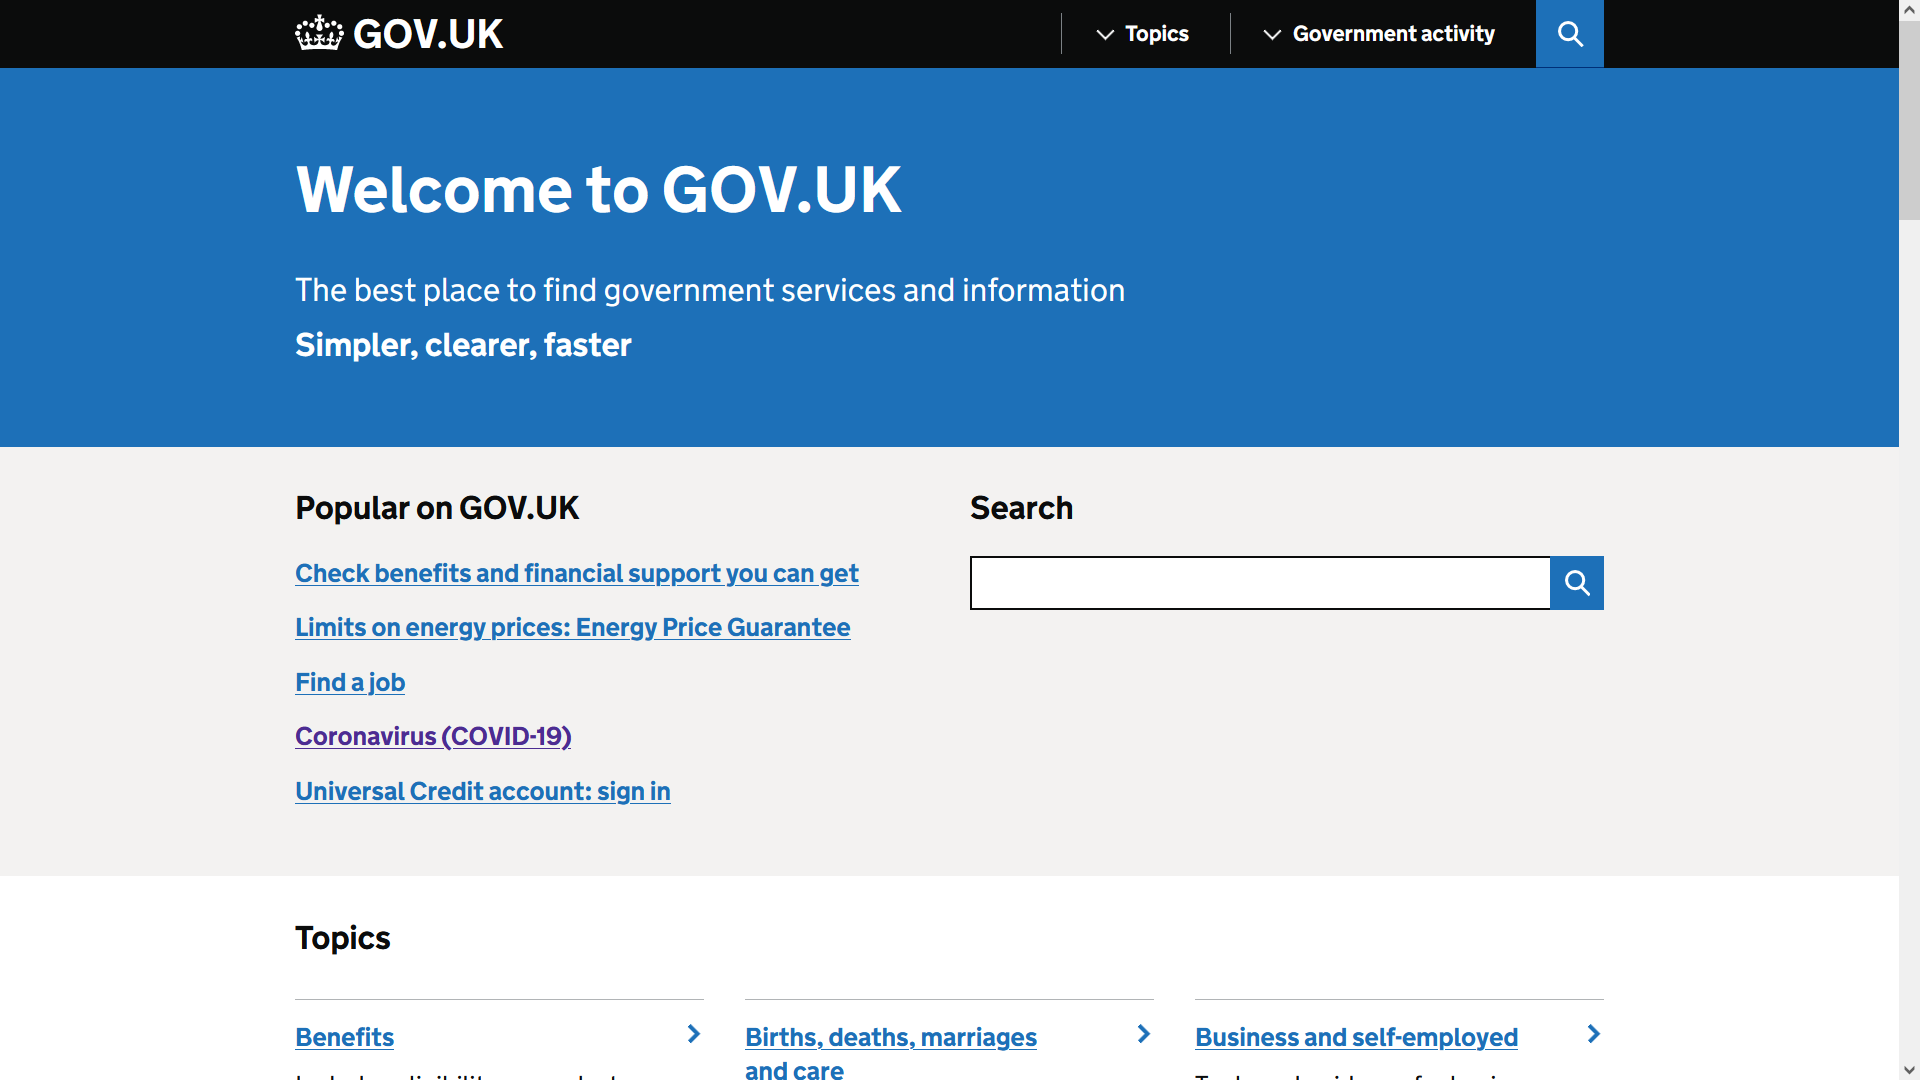
\includegraphics[keepaspectratio,width=\linewidth]
{images/gov}

\caption[www.gov.uk]
{%
This website is a good example of an accessible website.
}%
\label{fig:gov}
\end{figure}

\begin{figure}
\centering

\includegraphics[keepaspectratio,width=\linewidth]
{images/mirror}

\caption[www.mirror.co.uk]
{%
This website has quite a poor accessibility.
}%
\label{fig:mirror}
\end{figure}


\cleardoublepage
%----------------------------------------------------------------
%
%  File    :  text-only-browsers.tex
%
%  Author  :  Olli-Pekka Riikola, TU Graz, Austria
% 
%  Created :  2.12.2022
% 
%----------------------------------------------------------------


\chapter{Text-Only Browsers}

\section[tb-history]{A Quick Look to the History of Text-Only Browsers}
Originally, text browsers were the only way to browse the web. Also, back in the days, internet connetion speeds used to be much slower than today but similarly web sites were much simpler and it was possible to access them with even with the narrow bandwidth. After that there is now several powerful graphical web browsers for web users, but the text browsers still have some important usecases even they are quite old solution for web browsing. \parencite{best-text-browsers}. In addition, there is still a few promising text browser remaining and even receiving recent updates at least annually, and they are worth for have a look.

\section[tb-known]{Text-Only Browsers in use}
The header above might seems to be a bit exaggerating, but it is totally possible and sensible to use text browsers in daily basis. This is, because text browsers are lightweight softwares and still efficient on poor internet connection and they could actually help user to reduce distraction while browsing the web and that is why they could be a good choice for a browser even nowadays. The text browsers are designed to logically organize the content of the website rather than just to be ordinary web browser which gives the access to the site for a user. More than that, persons with no sight or who are partially impaired can more efficiently access website with text browser in combination with screen reader. And when talking about blind persons as a web users it is important to consider, that they obviusly can't see or otherwise access the actual graphical pieces of art, images, videos or other similar mediaformats in the website. \parencite[Chapter 2]{webbie} So, text browsers reduces the content that screen readers cannot read and that way they will make the web browsing more convenient for blind people.

\subsection[tb-problems]{Common Problems}
Event the layout of the site would be simple in text browser, it still is not simple in practice. According \textcite[Chapter 5]{webbie} the reason is presentation. People with sight can have advantage of very versatile navigation link list, but for a blind user it might be a struggle. It becomes a struggle at the point, when text browser try to present navigation bar as a list of links, and screen reader starts to read it - link by link, one by one. Luckily, there is an option to skip this navigation bar and go straight to the content, but only if the element is designed properly in the website. Otherwise text browser does not realize that there is a navigation bar, but it just present it like a list of links and user needs to handle it.

Another issue is empty attributes of element, like ALT attribute in IMAGE element. And of course this problem would quite easily be fixed by the programmer, specially with powerful accessibility checking tools, but sadly it is not always like that. So, since images are not relevant content for a person with no sight, it is very important that the ALT tag will tell, what is going on in that part of the website. Also, if image is for hyperlink, then it should also tell with ALT tag, where it will bring the user. \parencite[Chapter 5]{webbie}.

Perhaps, the most difficult issue in the terms of text browser, is dynamic content. Since most text browsers do not support JavaScript, some functionality is not available for the user in the site. This essentially means, that text browsers are not any more so convenient way to browse the web. But still, like mentioned in \ref*{tb-history}, there is few interesting text browser softwares available in the internet.

\section[tb-browsers]{Known Text-Only Browsers}
\subsection[tb-lynx]{Lynx}
Lynx is quite old text browser and it appears to be probably most well known one. But as it is in the \textcite{lynx} website, Lynx is a command line interface WWW client for Unix systems. Interesting sidenote could aslo be, that back in the years the Lynx has been a solution to build Campus Wide Information Systems. 
\subsection[tb-webbie]{WebbIE}
WebbIE is the one, which is designed to help visually impaired persons to access the web. They are dedicated to work in combination with screenreaders, like JAWS, WindowEyes, Thunder, NVDA and Narrator as mentioned in the \textcite{webbie-main} website. WebbIE runs on Windows, and it seems to be pretty much only choice for Windows users.
\subsection[tb-w3m]{W3M}
W3M is also a very handy text browser and it works as pager too, like 'more' or 'less' as it says in \textcite{w3m} website. It also works as text formatting tool from HTML to plain text.
\subsection[tb-links]{Links}
Another interesting and very nicely working text browser is Links which is school project from the days in 1999. But since then it has been kept up to date and many people are involved in the project and put effort to make Links more diverse. \parencite{links}. It runs on Unix.
\subsection[tb-others]{Others}
There is also few cases worth to mention, perhaps even if they are not in the same class with these ones mentioned above. However, there is a project called Browsh, which is a graphical text browser running on Linux. It supports JavaScript, so all functionality in the site should be accessed but it is still very early stage in the development. But it might be useful on poor internet connection. 

Another ones are more like plugins, but it is good to know, that there is still such. Chrome offers a plugin, which makes website like text site, but it seems to be somehow outdated and poor. More interesting and very well working built-in function is Firefox Reader-View. It just makes the website to be easier to read with removing distracting elements and making the content to be more cleary seen. This function can be activated just by pressing F9 in the Firefox browser and it works in several website.
\begin{figure}[tp]
    \centering
    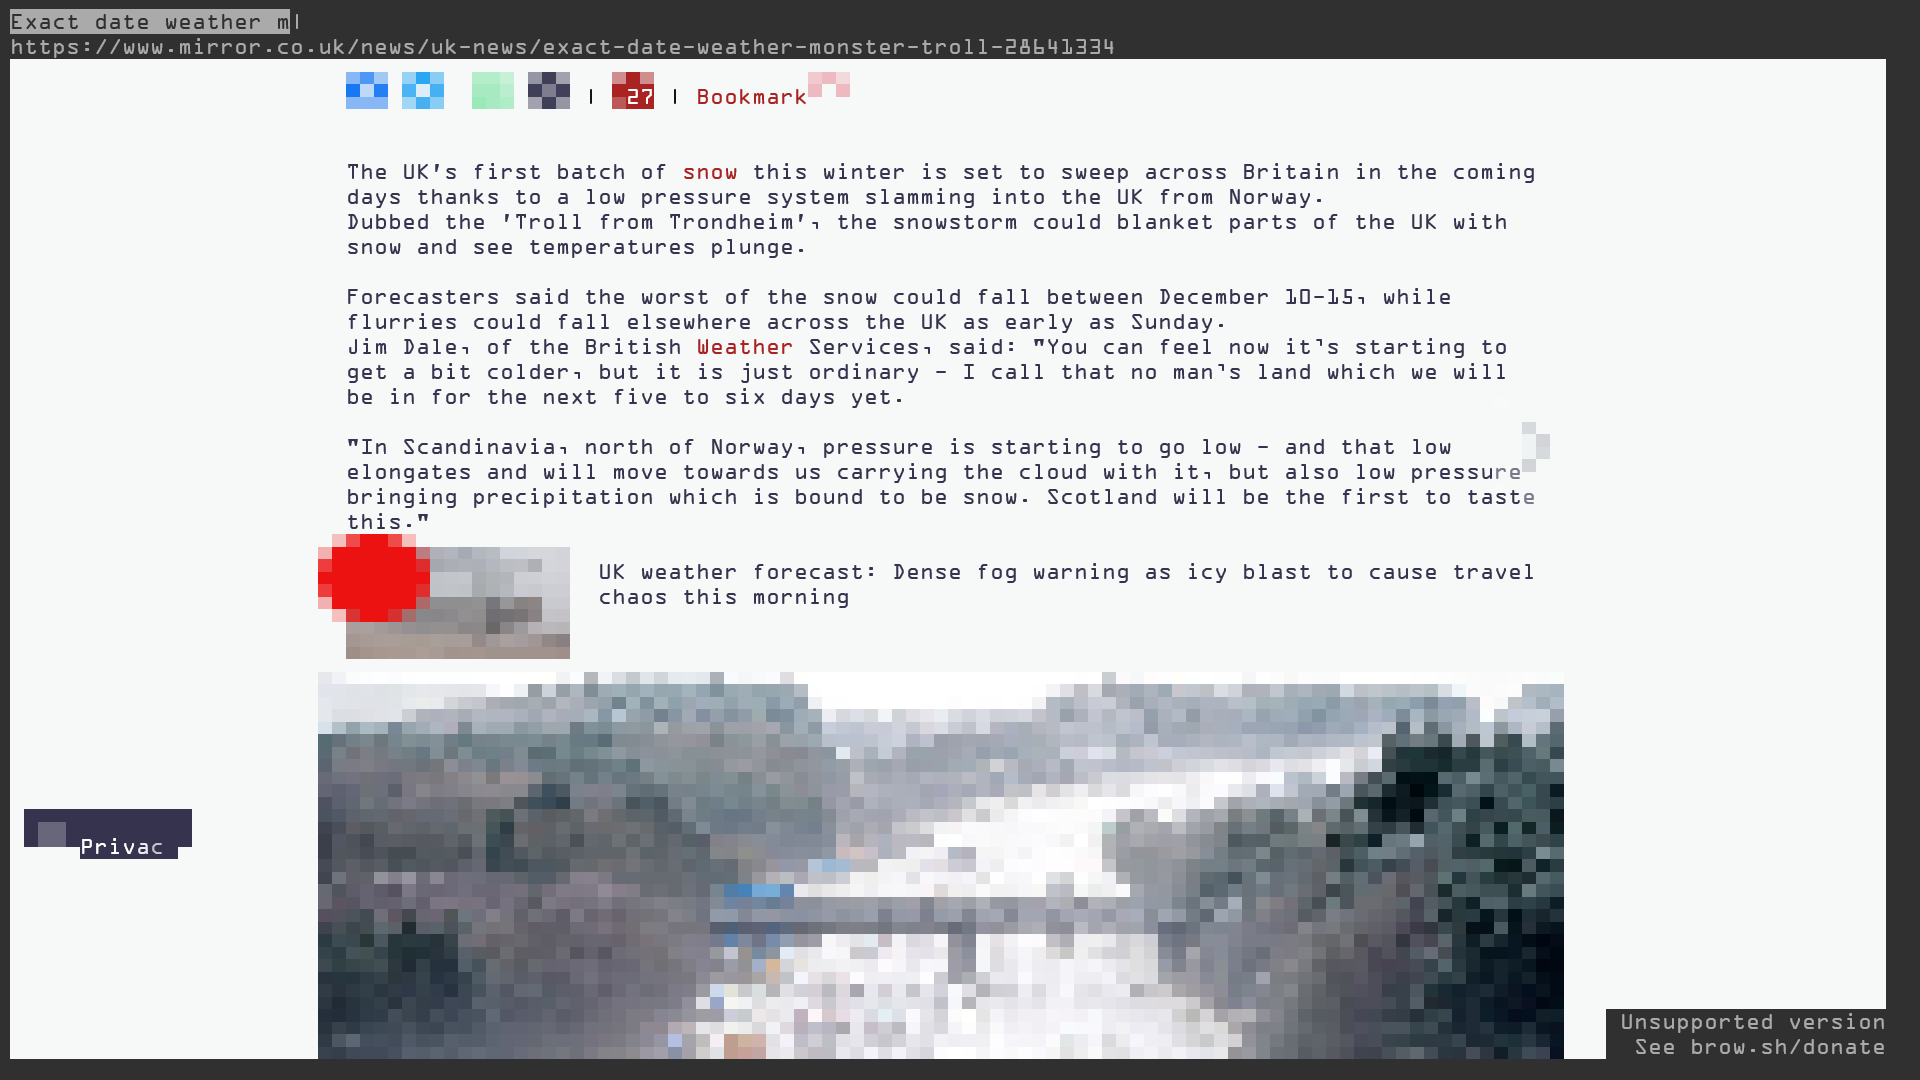
\includegraphics[keepaspectratio,width=\linewidth,height=\halfh]
    {images/browsh.png}
    
    \caption[Browsh grahical CLI browser]
    {%
    Browsing a web with Browsh in website gov.uk.
    }
    \label{fig:browsh}
\end{figure}
\begin{figure}[tp]
    \centering
    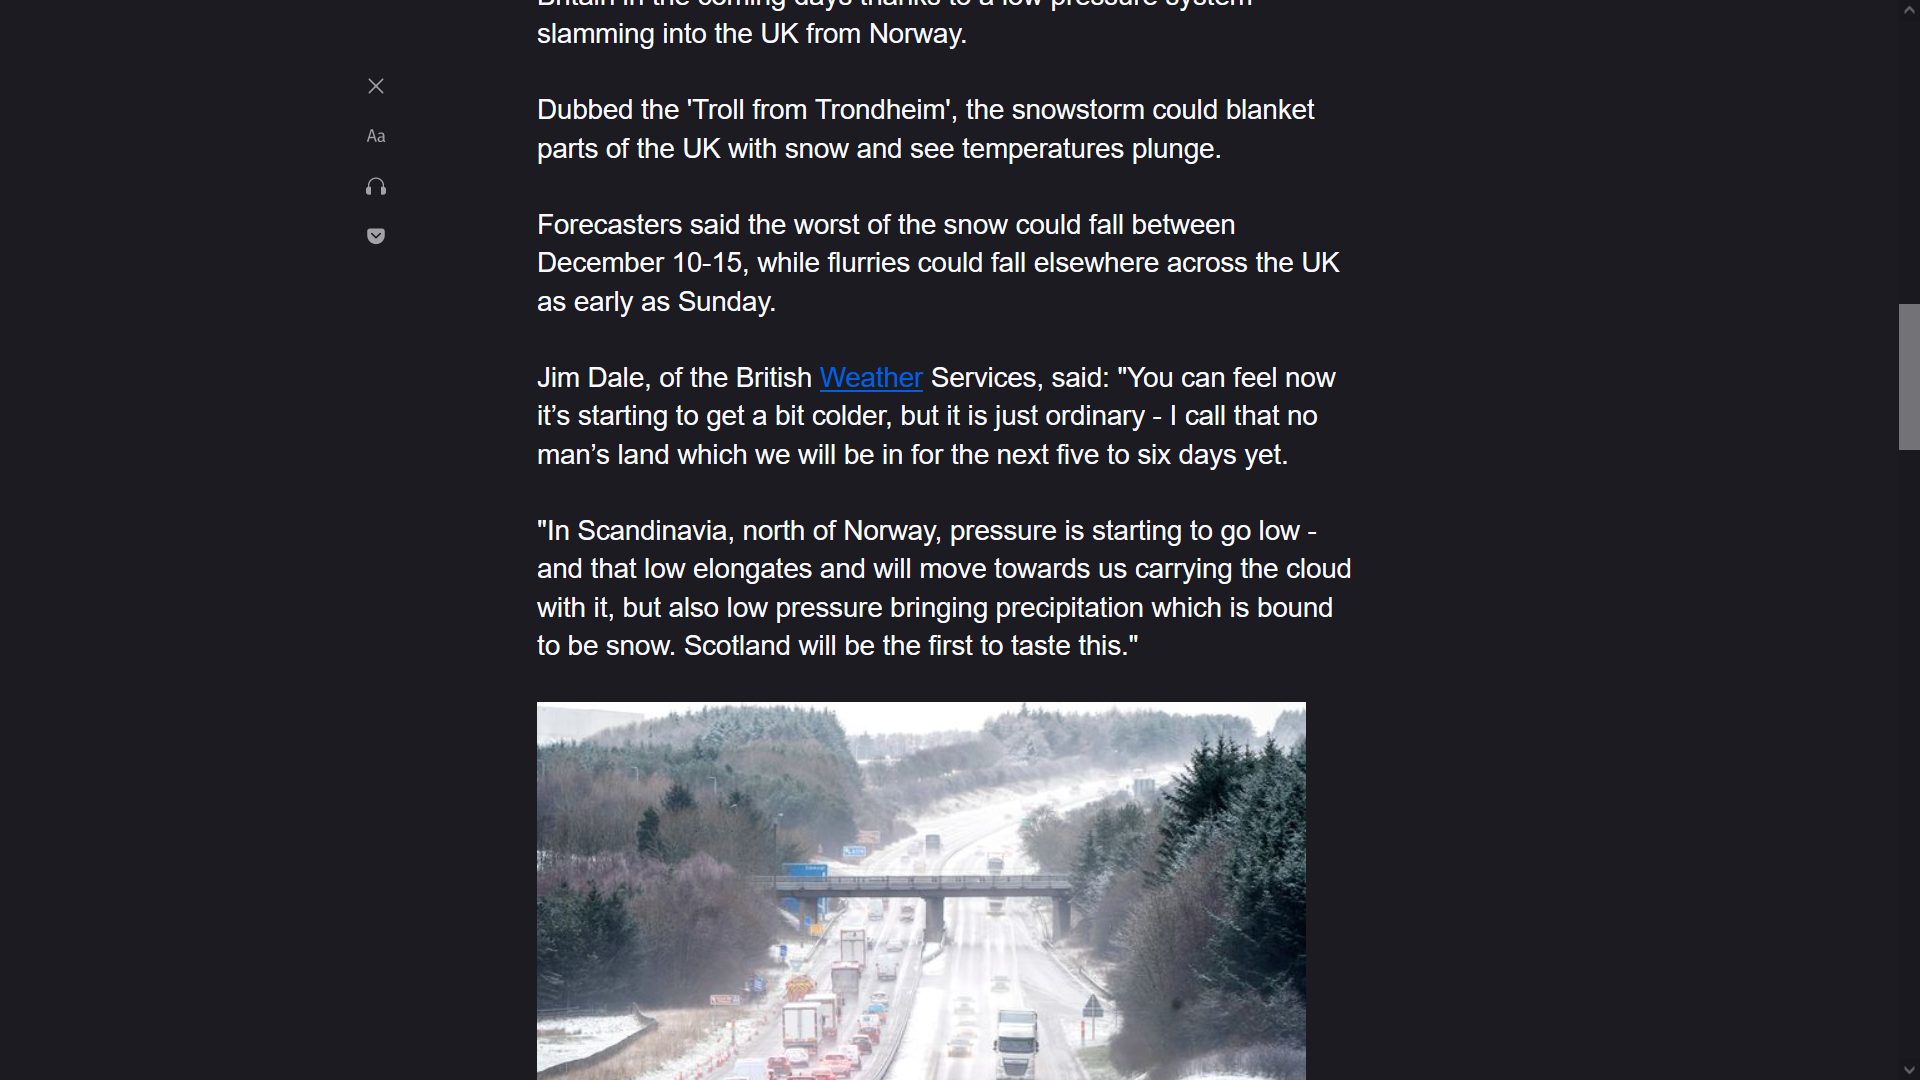
\includegraphics[keepaspectratio,width=\linewidth,height=\halfh]
    {images/reader-view.png}
    
    \caption[Firefox Reader-View]
    {%
    Browsing a web with Firefox Reader-View
    }
    \label{fig:firefox-rv}
\end{figure}
\section[tb-general]{Showcases and Data of Text Browsers}
In this section there is provided practical examples and an interesting data  of these text browsers. Due to siplicity of the text browsers, it is easy to get familiar with them to only watching a showcase video and comparing the screenshots below in the section \ref*{tb-screenshots}.
\subsection[tb-showcase]{}
There is showcase video in YouTube, where is shown what it looks like when browsing the web with the Lynx text browser. In the video it is shown two examples gov.uk and mirror.co.uk, which represents an examples of good and bad web accessibility. Both videos are quite similar in structure, just tabbing through the sites and entering the links, but that way it is easy to recognize the probles with the first glance in the mirror.co.uk website. Link to the showcase video is provided in reference \textcite{tb-showcase}.
\subsection[tb-screenshots]{Screenshots of Text Browsers}
Following images presents how efficient a text browsers actually could be. In the case of mirror.co.uk, even if there is plenty of images and advertisements, the text browsers are able to present the content somehow sensible. In this area, most interesting examples is Lynx and WebbIE. Others are more or less similar than the Lynx - only thing to consider is, that W3M and Links works responsively inside of CLI, Lynx does not. 

\begin{figure}[tp]
    \centering
    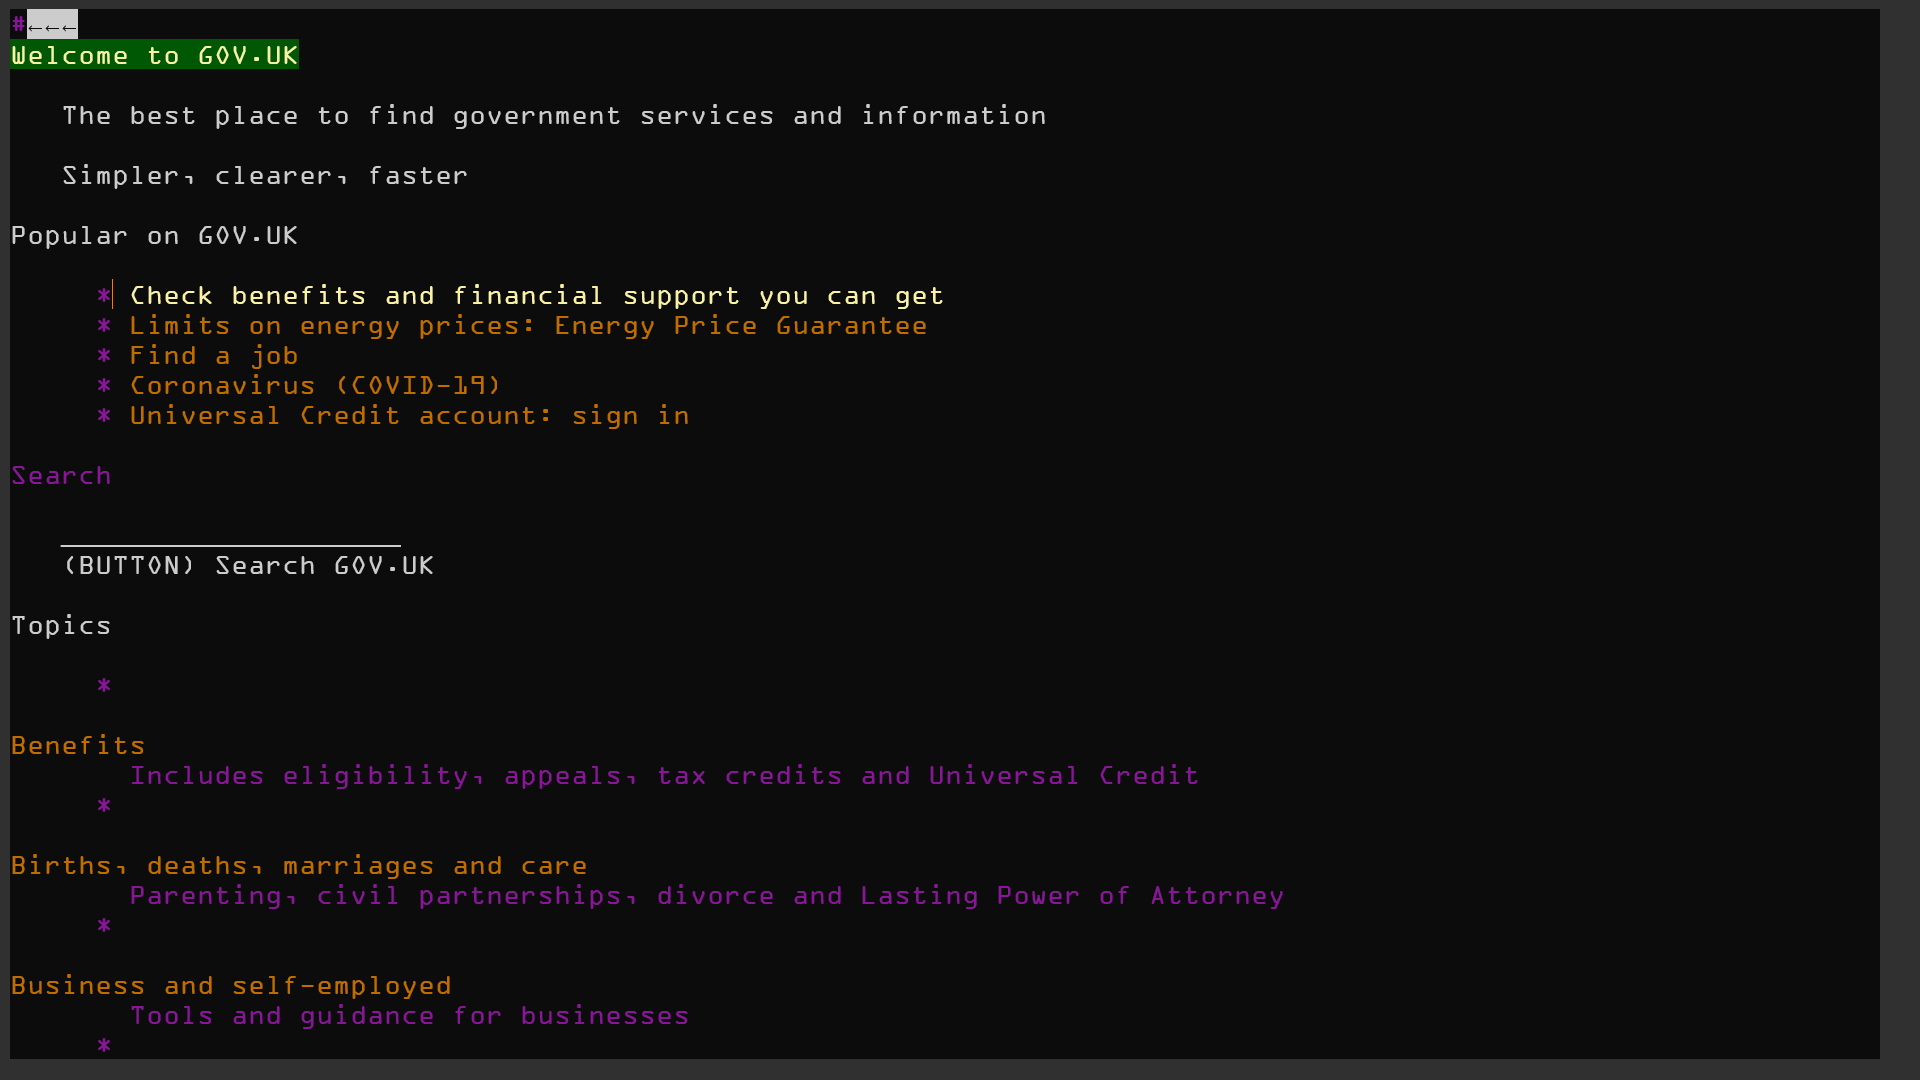
\includegraphics[keepaspectratio,width=\linewidth,height=\halfh]
    {images/lynx-gov}
    
    \caption[Lynx browser]
    {%
    Browsing the gov.uk website
    }
    \label{fig:lynx-gov}
\end{figure}

\begin{figure}[tp]
    \centering
    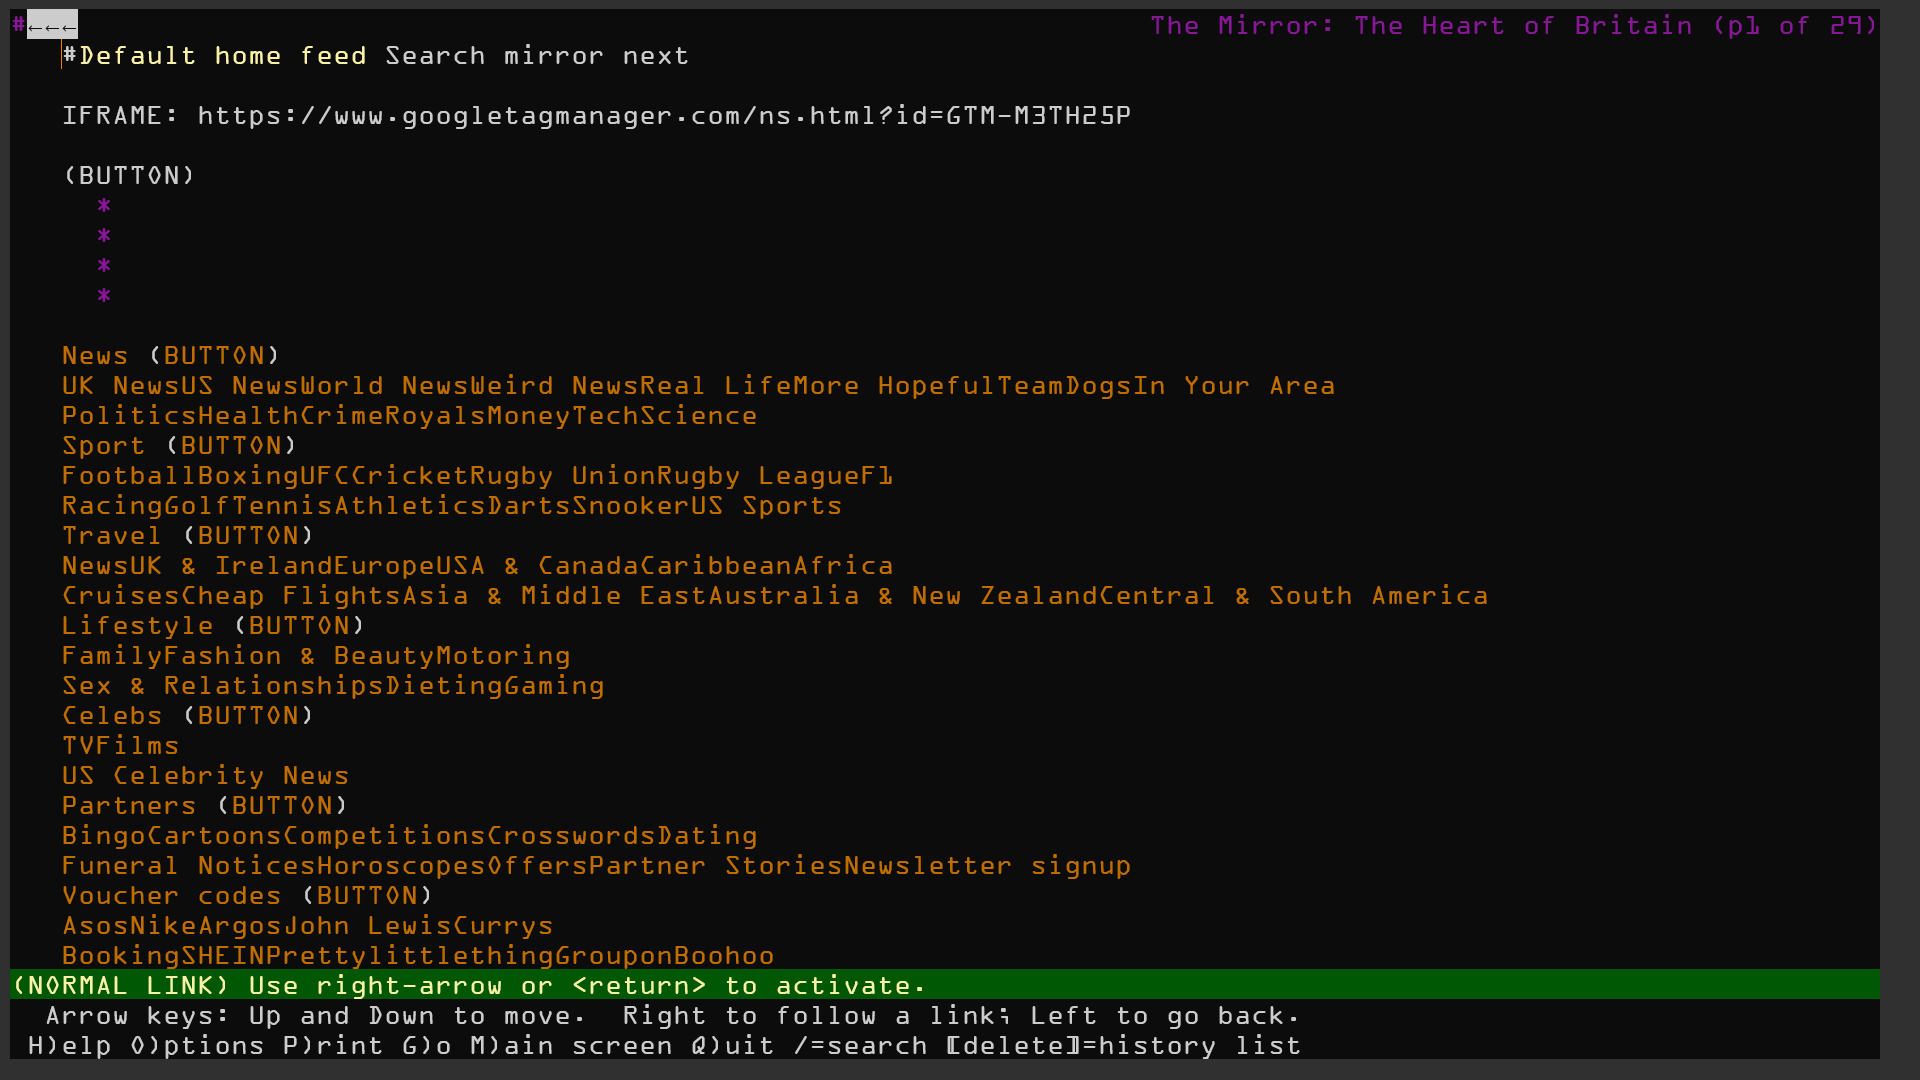
\includegraphics[keepaspectratio,width=\linewidth,height=\halfh]
    {images/lynx-mirror}
    
    \caption[Lynx browser]
    {%
    Browsing the mirror.co.uk website
    }
    \label{fig:lynx-mirror}
\end{figure}

\begin{figure}[tp]
    \centering
    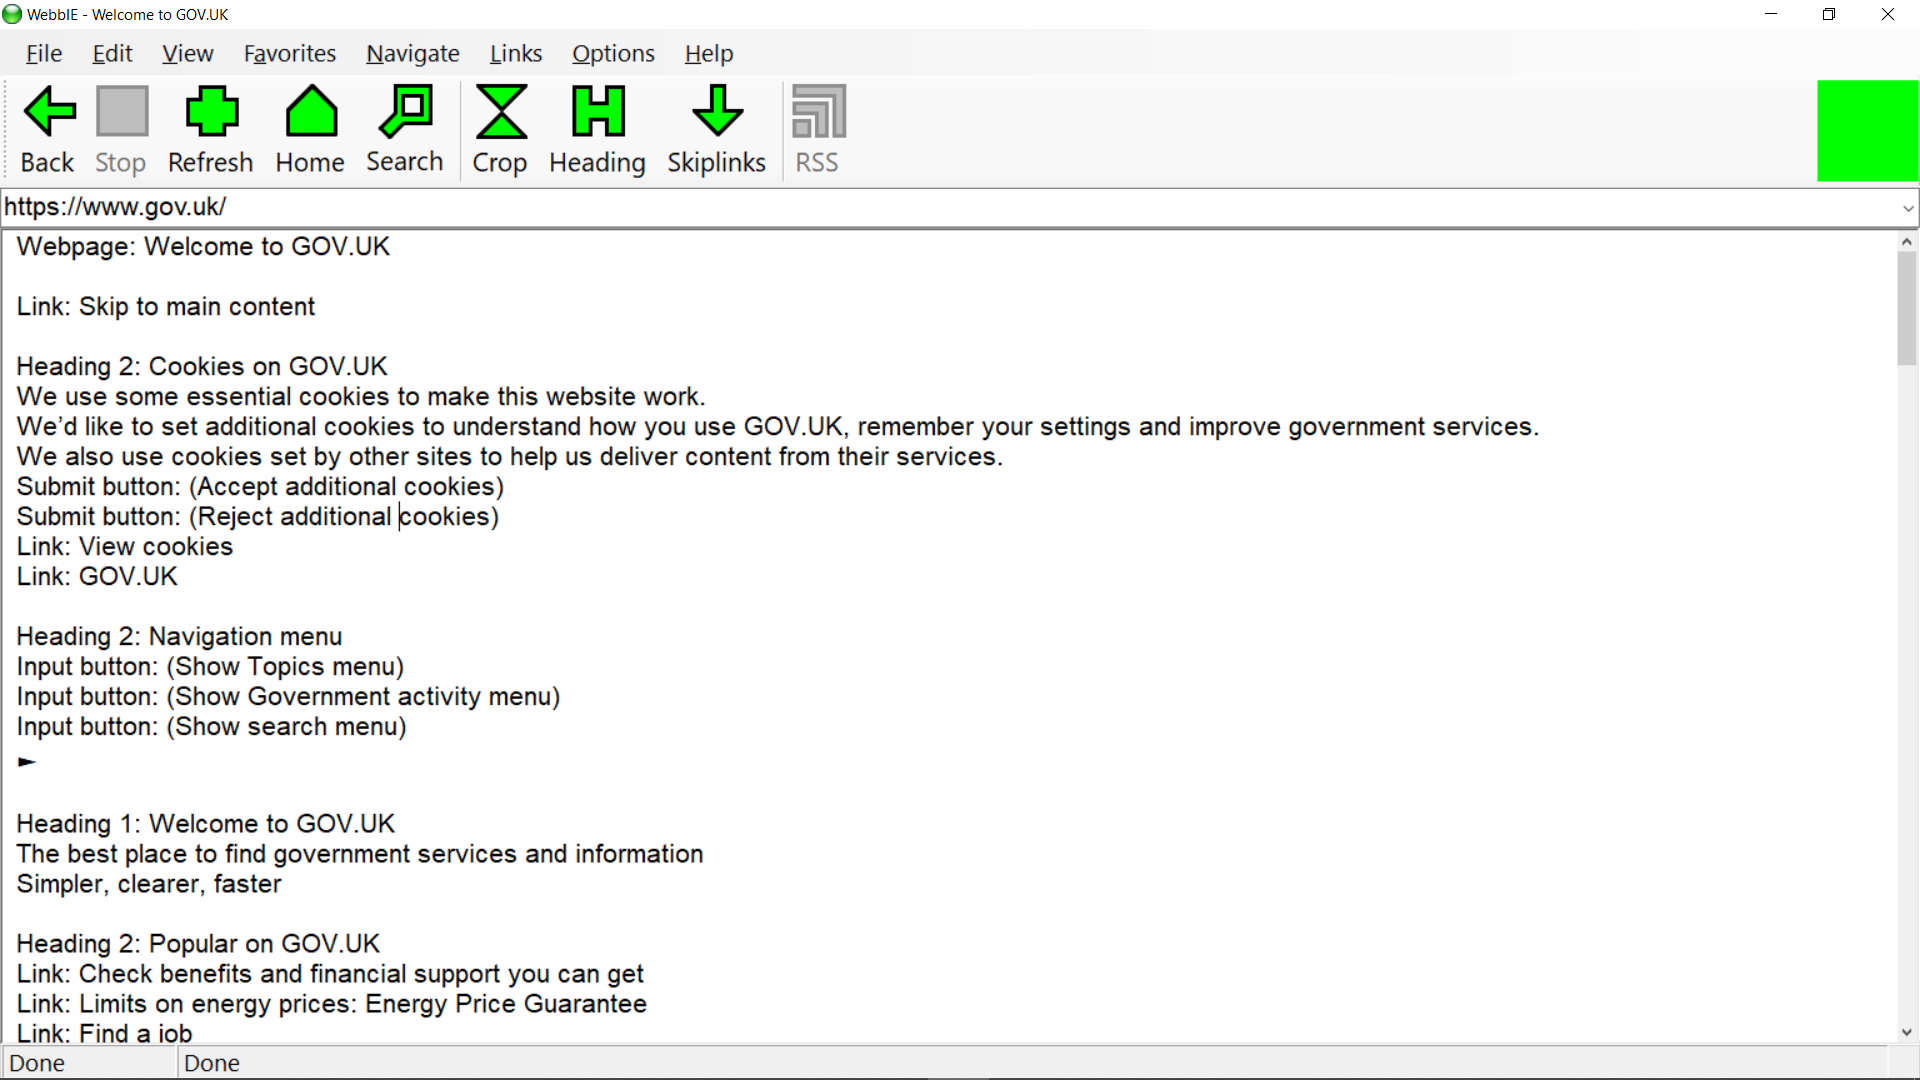
\includegraphics[keepaspectratio,width=\linewidth,height=\halfh]
    {images/webbie-gov}
    
    \caption[WebbIE browser]
    {%
    Browsing the gov.uk website
    }
    \label{fig:webbie-gov}
\end{figure}

\begin{figure}[tp]
    \centering
    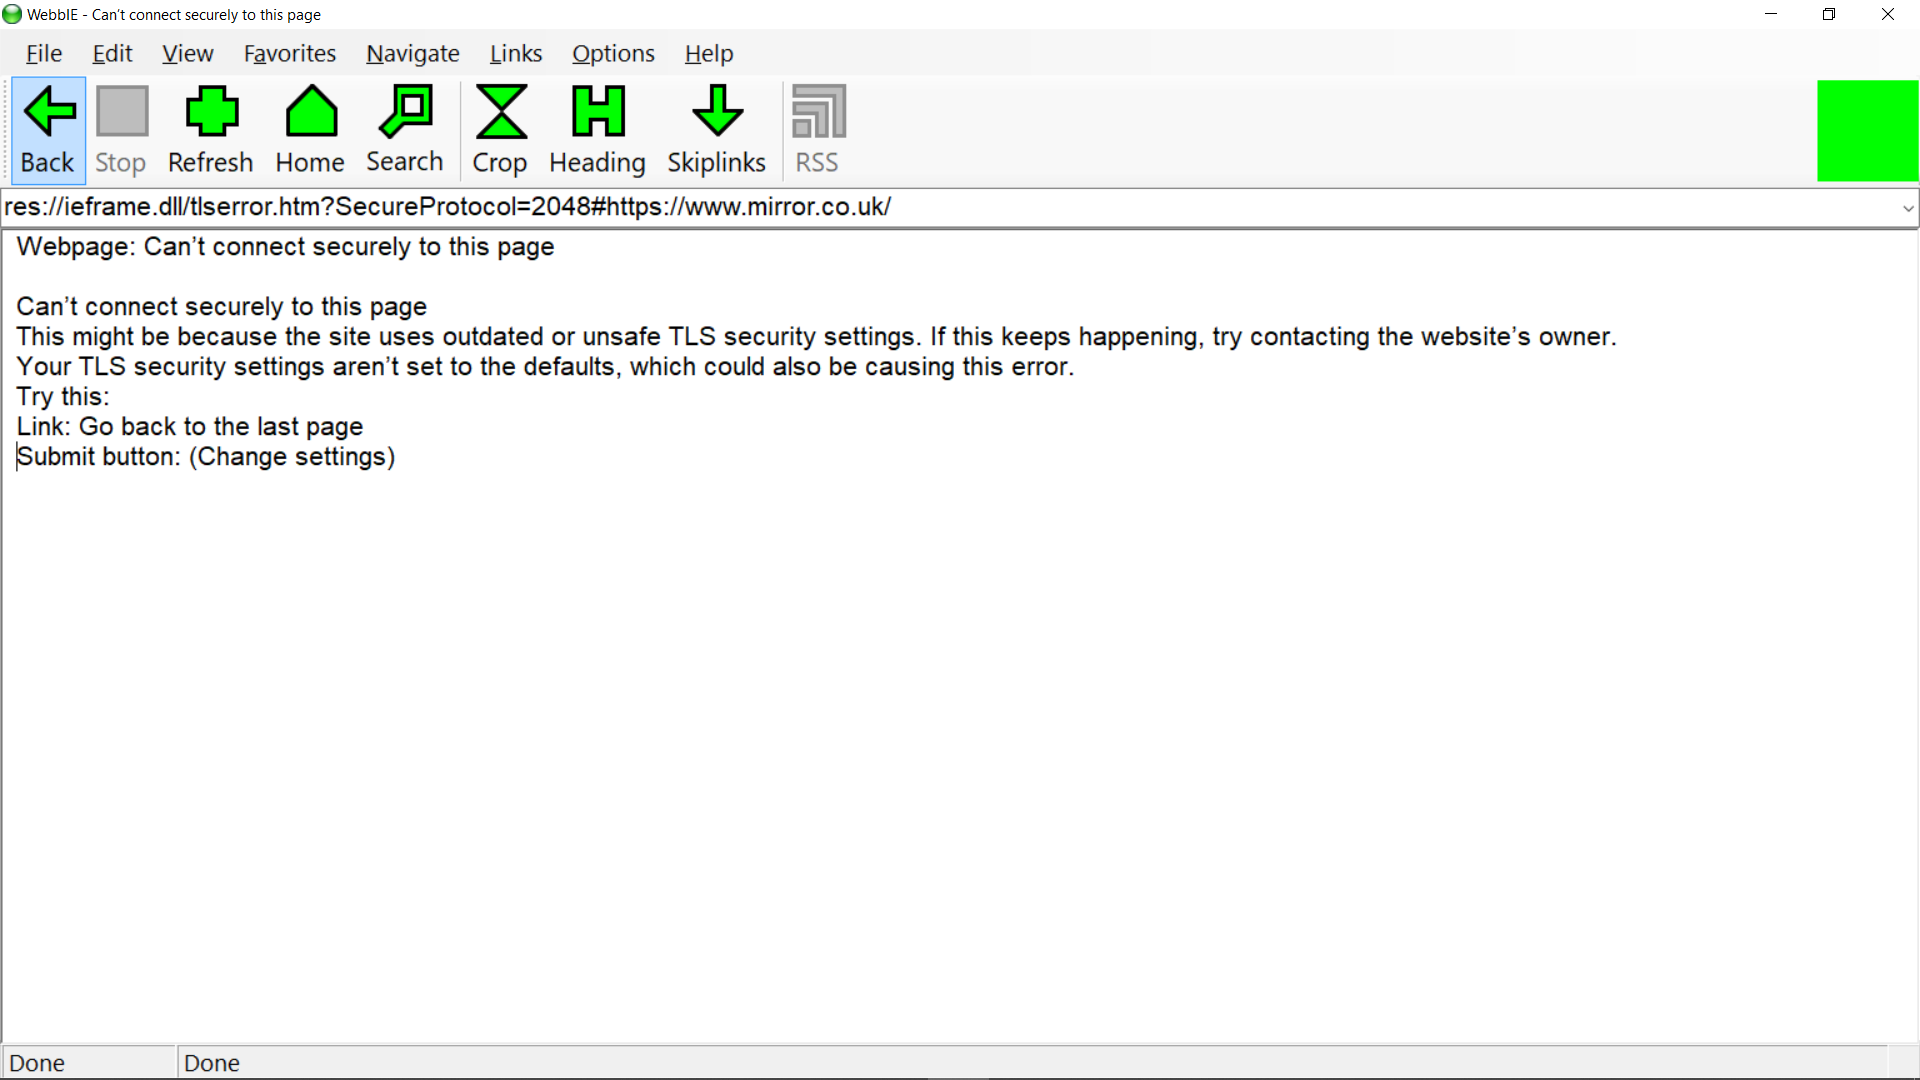
\includegraphics[keepaspectratio,width=\linewidth,height=\halfh]
    {images/webbie-mirror}
    
    \caption[WebbIE browser]
    {%
    Browsing the mirror.co.uk website
    }
    \label{fig:webbie-mirror}
\end{figure}

\subsection[tb-tables]{Basic Data About Text-Only Browsers}
\begin{table}[tp]
    \tablestretch
    \rowcolors{2}{}{tablerowcolour}
    \centering
    \begin{tabularx}{\linewidth}
    {>{\kern-\tabcolsep}lllXX<{\kern-\tabcolsep}}
    \toprule
    \textbf{Browser} & \textbf{Last update} & \textbf{System} & \textbf{Licence} & \textbf{No. of lang.} \\
    \midrule
    JAWS & 25. 10. 2022 & Windows & Commercial & 10 \\
    %
    NVDA & 1. 3. 2022 & Windows & Free and open-source & 63 \\
    %
    VoiceOver & 24. 10. 2022 & iOS, macOS & Free & 64 \\
    %
    Narrator & 2020 & Windows & Free & 49 \\
    %
    TalkBack & 27. 10. 2022 & Android & Free and open-source & 63 \\
    \bottomrule
    \end{tabularx}
    
    \caption[Screen Readers Information]
    {
    Information of text browsers
    }
    \label{tab:text-browsers-info}
    \end{table}

\cleardoublepage
%----------------------------------------------------------------
%
%  File    :  survey-intro.tex
%
%  Author  :  Keith Andrews, IICM, TU Graz, Austria
% 
%  Created :  27 May 1993
% 
%  Changed :  16 Nov 2010
% 
%----------------------------------------------------------------


\chapter{Screen Readers}

Screen readers are software applications, primarily used by visually impaired people. Screen readers convert web content (text, buttons, images, and other elements) into speech or braille output. Screen readers attempt to convey what visually non-impaired people see on a display via non-visual means like text-to-speech, sound icons, or a braille device.

In May - June 2021, WebAIM surveyed the  preferences of screen reader users. They received 1568 valid responses. Figure~\ref{fig:screen-readers-piechart} shows the primary screen readers preferences. The majority of users use JAWS and NVDA screen readers as their primary screen readers. Figure~\ref{fig:screen-readers-line} shows historical trends for primary screen reader usage. After a decade of decreases in primary usage, JAWS is once again the most used screen reader, with NVDA and VoiceOver both decreasing in primary usage over the last two years.

In this paper, we focus on JAWS, NVDA, VoiceOver, Narrator, and TalkBack screen readers. They are further described in the sections below.

\begin{figure}[tp]
\centering
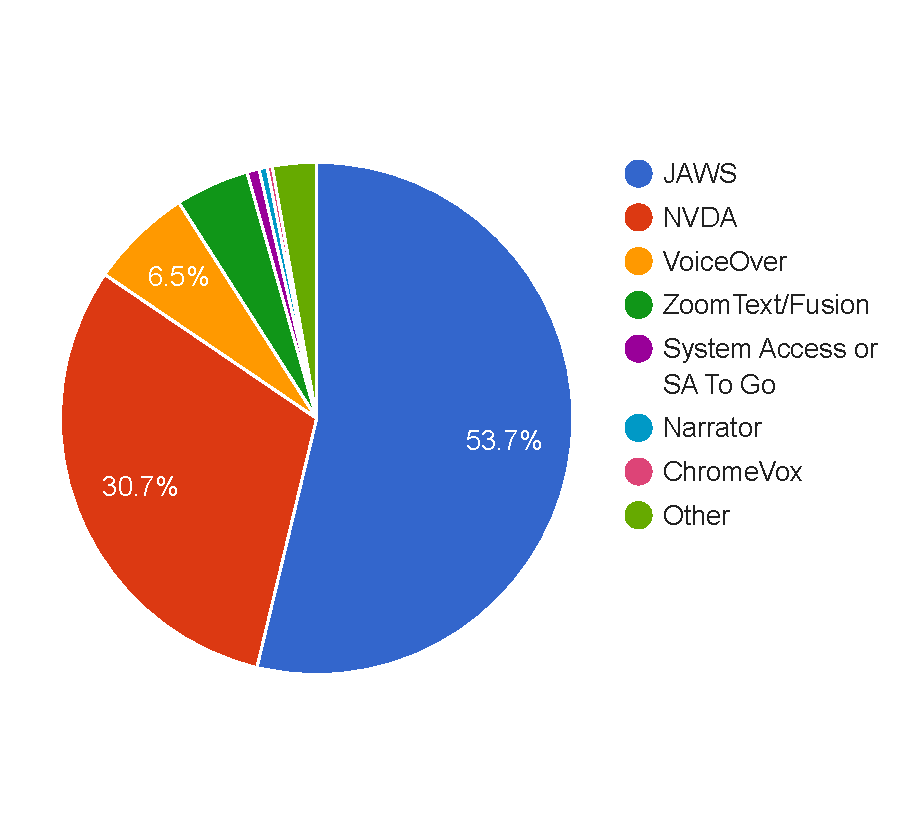
\includegraphics[keepaspectratio,width=\linewidth,height=\halfh]
{images/screen-readers-piechart.pdf}

\caption[Primary Screen Reader]{
Primary screen reader.
\imgcredit{Image extracted from WebAIM. ©2022 WebAIM.}
}
\label{fig:screen-readers-piechart}
\end{figure}

\begin{figure}[tp]
\centering
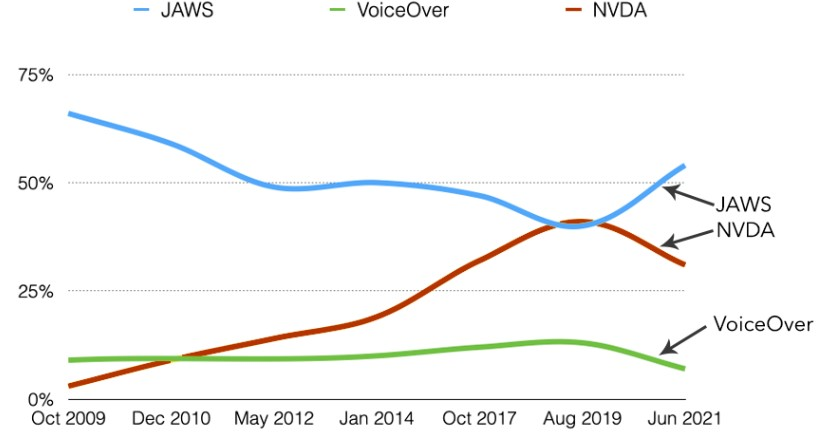
\includegraphics[keepaspectratio,width=\linewidth,height=\halfh]
{images/screen-readers-line.jpg}

\caption[Historical Trends for Primary Screen Reader]{
Historical trends for the primary screen reader.
\imgcredit{Image extracted from WebAIM. ©2022 WebAIM.}
}
\label{fig:screen-readers-line}
\end{figure}




\section{JAWS}
JAWS is the most popular screen reader for Windows computers, however, it has a learning curve. JAWS has a lot of shortcuts and hotkeys that a user has to get used to in order to operate JAWS efficiently. JAWS has the most configurable options among the reviewed screen readers. JAWS is only available as paid software, either as an enterprise or single-use package (90 EUR a year or approximately 900 EUR as a one-time purchase). JAWS demands a lot of the computer's RAM and can occasionally slow the computer down. JAWS supports 10 languages.

\section{NVDA}

NVDA is the second most popular screen reader for Windows computers. NVDA is available as free and open-source software. NVDA is a good free alternative to JAWS, however, it is not as configurable as JAWS. NVDA has a lot of shortcuts and hotkeys that a user has to get used to in order to operate NDVA efficiently. NVDA supports 63 languages.

\section{VoiceOver}

VoiceOver is free and comes included with all Apple products. VoiceOver requires no installation or setup. VoiceOver is user-friendly and configurable. The learning curve takes some effort since VoiceOver is not operated the same way as typical mobile phone users are used to. Voice is operated by multiple special gestures (for example double finger drag, triple finger drag). VoiceOver supports 64 languages.

\section{Narrator}

Narrator is free and comes included with the Windows operating system. Narrator requires no installation or setup. Narrator has some shortcuts and hotkeys, but not as many as JAWS and NVDA. Narrator offers limited functionality with web  browsers and web apps, especially with navigation and deeper levels of the Windows operating system. Narrator supports 49 languages.

\section{TalkBack}

TalkBack is free and open-source. TalkBack comes included with the Android operating system. TalkBack requires no installation or setup. TalkBack is user-friendly, however, the learning curve takes some effort, since TalkBack is not operated the same way as typical mobile phone users are used to. TalkBack is operated by multiple special gestures (for example swipe left then right). TalkBack supports 63 languages.

\section{Showcase Videos}
We recorded showcase videos for each screen reader. We used the screen readers on the UK government site~\parencite{GovUK}, which is a good example of web accessibility site, and on the Mirror newspaper site~\parencite{MirrorUK}, which is a bad example of web accessibility site.
Showcase videos for JAWS (\parencite{JAWS_gov}, \parencite{JAWS_mirror}), NVDA (\parencite{NVDA_gov}, \parencite{NVDA_mirror}), VoiceOver (\parencite{VoiceOver_gov}, \parencite{VoiceOver_mirror}), Narrator (\parencite{Narrator_gov}, \parencite{Narrator_mirror}), and TalkBack (\parencite{TalkBack_gov}, \parencite{TalkBack_mirror}) are available online.

\section{Screen Readers Conclusion}

A comparison of information can be seen in  Table~\ref{tab:screen-readers-info}. All screen readers in question, except Narrator, are maintained regularly. JAWS, NVDA, and Narrator are available on Windows, VoiceOver is available on iOS and macOS, and TalkBack is available on Android. JAWS supports 10 languages while other screen readers support between 49 and 64 languages. JAWS is the only screen reader available as paid software while other screen readers are available as free software (NVDA and TalkBack are also open-source). Windows users have 3 options: JAWS, NVDA, and Narrator. The most popular paid option for Windows is JAWS, and the most popular free option for Windows is NVDA. iOS and macOS users can use VoiceOver, and Android users can use TalkBack.

\begin{table}[tp]
\tablestretch
\rowcolors{2}{}{tablerowcolour}
\centering
\begin{tabularx}{\linewidth}
{>{\kern-\tabcolsep}lllXX<{\kern-\tabcolsep}}
\toprule
\textbf{Screen reader} & \textbf{Last update} & \textbf{System} & \textbf{Licence} & \textbf{No. of lang.} \\
\midrule
JAWS & 25. 10. 2022 & Windows & Commercial & 10 \\
%
NVDA & 1. 3. 2022 & Windows & Free and open-source & 63 \\
%
VoiceOver & 24. 10. 2022 & iOS, macOS & Free & 64 \\
%
Narrator & 2020 & Windows & Free & 49 \\
%
TalkBack & 27. 10. 2022 & Android & Free and open-source & 63 \\
\bottomrule
\end{tabularx}

\caption[Screen Readers Information]
{
Screen readers information
}
\label{tab:screen-readers-info}
\end{table}




\cleardoublepage
\chapter{Browser Extensions for Accessibility Auditing}

\label{chap:Intro}

Using browser extensions is one way to audit the accessibility of websites.
This paper evaluates five different extensions for accessibility auditing: axe DevTools, Accessibility Insights for Web, Google Lighthouse, Siteimprove and WAVE.
Three of the tools we have selected for this paper use the \emph{axe-core} library, which is an open-source accessibility engine for automated web UI testing.
As a result, many of the tools will give similar results and the main difference between the extensions is how the list of accessibility issues is presented and what additional features are offered.
The library allows accessibility auditing to Web Content Accessibility Guidelines (WCAG) 2.0 and 2.1 on the levels A and AA.

Most of the browser extensions evaluated in this paper are completely free.
Only one of the tools evaluated in this paper offers a paid version of the extension with additional features.

\begin{table}[tp]
\tablestretch
\rowcolors{2}{}{tablerowcolour}
\centering
\begin{tabularx}{\linewidth}
{>{\kern-\tabcolsep}lllXX<{\kern-\tabcolsep}}
\toprule
\textbf{Extension} & \textbf{Browser} & \textbf{Licence} & \textbf{Downloads\footnotemark}
\\
\midrule
axe DevTools & Chrome, Edge & Free, commercial & 210000 \\
%
Accessibility Insights for Web & Chrome, Edge & Free, open-source & 120000 \\
%
Google Lighthouse & Chrome (built-in) & Free, open-source & 900000\footnotemark \\
%
Siteimprove Accessibility Checker & Chrome, Firefox, Edge, Opera & Free & 30000 \\
%
WAVE Evaluation Tool & Chrome, Firefox, Edge & Free & 520000 \\
\bottomrule
\end{tabularx}
\caption[Browser Extensions Information]
{
Browser extensions information \\
% TODO: Figure out how to use \footnotetext here
\textsuperscript{1}\text{Data collected from Chrome Web Store, Opera Addons, Firefox Add-ons and Microsoft Edge Add-ons.} \\
\textsuperscript{2}\text{Google Lighthouse is built-in into Google Chrome, so the actual number of users may be significantly higher.}
}
\label{tab:browser-extensions-info}
\footnotetext{test}
\end{table}

\section{axe DevTools}
Axe DevTools is a tool for auditing accessibility developed by Deque Systems Inc.
The browser extension is based on the \emph{axe-core} underlying library for auditing the accessibility, but also offers some additional stricter audit rules compared to the base \emph{axe-core} library, allowing validation according to WCAG 2.1 AAA.
The extension is available for Chrome and Edge.
The Deque website contains a link to the axe DevTools extension for Firefox, but at the time of writing this paper it does not seem to work.

There are three different plans available, Free, Pro and Enterprise.
The free version has a limited set of features and mostly consists of only the automated testing of accessibility.
The Pro version costs \$40 per month and offers additional features, such as guided manual tests, partial accessibility testing and exporting of accessibility issues.
Lastly, the Enterprise version of axe DevTools offers even more features, for example CI/CD integration and custom rules.


\section{Accessibility Insights for Web}
Accessibility Insights for Web is a browser extension for accessibility auditing using Chrome or Edge.
The extension offers two different audit methods, automated checking, known as FastPass, and manual assessment.
The FastPass automated check provides accessibility auditing using the the axe-core library.
The accessibility issues are then visible in a list and can be exported as an HTML report or directly to GitHub Issues or Azure Boards for easy integration in the development process.
Another feature available in the extension is the visualization of accessibility issues directly on the web page.
This allows scrolling the web page to see where accessibility issues occur .
The manual assessment in the browser extension consists of extensive step-by-step instructions for auditing the accessibility manually.
Of the browser extensions evaluated in this paper, Accessibility Insights for Web is the only free tool to offer support for manual testing.


\section{Google Lighthouse}
Google Lighthouse is a the most popular tool for auditing accessibility, which is included in Google Chrome.
Lighthouse, like the previous browser extensions, is also based on the \emph{axe-core} library.
For auditing accessibility, Lighthouse offers a relatively basic set of features, and relies heavily on integration with Chrome DevTools and external references for accessibility issue descriptions.
Accessibility issues are presented as a list of what accessibility checks have passed and which ones have failed.
The user can then see descriptions about the accessibility issues and see where in the HTML code they occur.
Reports of the accessibility audit can be saved as JSON.

\section{Siteimprove Accessibility Checker}
Siteimprove Accessibility Checker is the least used accessibility audit browser extension out of the extensions in this survey.
The extension presents the accessibility issues, where you can expand each issue to read the description of it and highlight the element on the web page.
Some features that the extension offers, that the other extensions do not offer is simulation of color blindness and excellent filtering of accessibility issues.
The list of issues can be filtered by difficulty, role, WCAG level and HTML element type.
However, one feature that is not offered is the possibility of exporting the audit report.

\section{WAVE Evaluation Tool}
The WAVE evaluation tool is another extension for auditing accessibility, supporting Chrome, Firefox and Edge.
The extension functions somewhat differently than the other extensions, as the tool is embedded directly on the web page.
It then inserts icons for elements that fail or succeed in the accessibility checks.
The user can then scroll the web page and click the icons to learn more about the accessibility issue.

\section{Showcase videos}
For each of the browser extension, we have recorded videos to showcase the extension and their features.
Using each extension, we performed an accessibility audit of http://www.gov.uk/ http://www.mirror.co.uk/.
The showcase videos for axe DevTools \parencite{axe_ext_vid}, Accessibility Insights for Web \parencite{aiweb_ext_vid}, Google Lighthouse \parencite{lighthouse_ext_vid}, Siteimprove Accessibility Checker \parencite{siteimprove_ext_vid}, WAVE Evaluation tool are available online \parencite{wave_ext_vid}.

\section{Browser Extensions Conclusion}
TODO: add conclusion



\cleardoublepage
%----------------------------------------------------------------
%
%  File    :  survey-intro.tex
%
%  Author  :  Keith Andrews, IICM, TU Graz, Austria
% 
%  Created :  27 May 1993
% 
%  Changed :  16 Nov 2010
% 
%----------------------------------------------------------------


\chapter{Web Tools For Accessibility Audits}

\label{chap:WebTools}



Web tools for accessibility audits provide core auditing functionality
to anyone interested. The amount of tools in this category is large,
and most of these tools come to the same conclusions for an audited
web page regardless of the level of detail. This is attributed to
several factors, one being that many of these web tools are using the
same core library to assess the accessibility of a given website. In
the case of this survey, the used library is called axe-core, which is
provided by the Deque company.

In this survey, the tools that are inspected closely are but a
fraction of the tools that are currently available on the web. The
chosen tools were selected in a way, which enables a closer look at
tools that run with the axe core library and without. Additionally,
the selection also tries to show the different qualities of each
choice and what can be expected when someone tries to use these tools
online.

In this survey, our selection of web tools for accessibility audits
consists of the following: Accessi, WAVE, and Page Speed Insights
which is the web tool equivalent to the Lighthouse browser
extension. All of the mentioned web tools will be discussed in further
detail in the following sections. For each of these three tools, there
were also videos created, which demonstrates the features and the
functionality of each of the tools. The videos also give a quick
overview of the metrics that were used to determine the accessibility
of the tested websites.




\section{Accessi}

Accessi \parencite{Accessi} is one of the websites that were used to
assess the accessibility of the two test pages. Accessi is a website
that offers a free accessibility test to its users. It works according
to the Web Content Accessibility Guidelines (WCAG) standard. This can
be further refined while using the tool by a choice of the 2.0 version
of this standard or its 2018 renewed 2.1 version.  The website will
analyze the target test website and give a basic rating between
0-100\% telling the user the state of compliance of the test
site. Through an automated test, further metrics are detected, one
example being a statistical analysis of the found issues on the web
page. Accessi ranks these issues in three categories: High impact,
medium impact, and low impact. The high-impact issues are the most
obvious and intrusive ones, descending in severity, followed by medium
and low. All the issues that are detected by the automated test run
will additionally be listed, described, and enhanced with
examples. The feature that makes Accessi stand out from its
competitors is the ability to export all of the aforementioned
findings in PDF or CSV format, giving the user a form of a To-Do list
or a fixed statement that they could work on if they would be looking
towards improving the accessibility of their web site. An example of
the graphical interface of Accessi can be seen in
Figure~\ref{fig:accessi}.



\begin{figure}[tp]
\centering
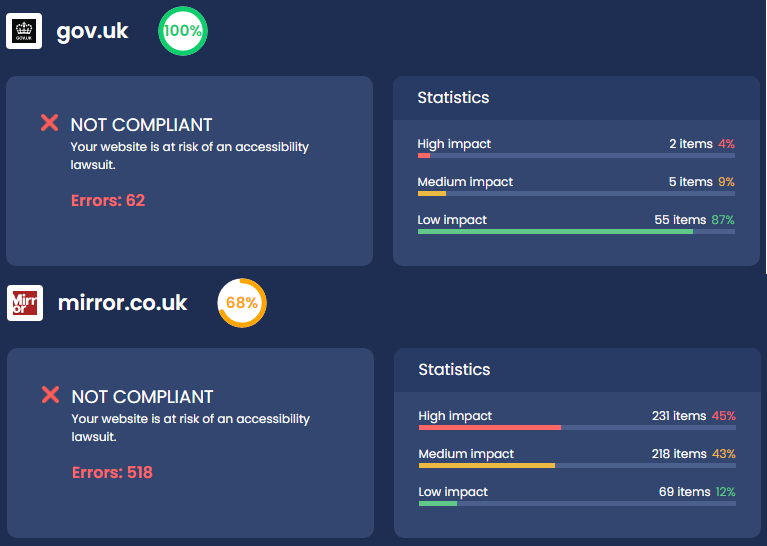
\includegraphics[keepaspectratio,width=\linewidth,height=\halfh]
{images/accessi.png}

\caption[Accessi Overview]
{%
Accessi web tool header showing an overview for each test site.
}
\label{fig:accessi}
\end{figure}





\section{WAVE}

WAVE \parencite{WAVE_web} is a tool provided by the company WebAim. As
the tools described in this survey its purpose is to assess the
accessibility of a website. WAVE offers a different take on the user
interaction with a website which is subject to an accessibility
test. The user is offered an interactive web tool, which embeds itself
in the test website which is being surveyed.  This embedded interface
gives the user the ability to interactively inspect all the errors and
warnings that are produced for a given website. The user is given the
ability to click on icons which are attatched to elements of the test
site, clearly outlining which element is considered non-compliant with
accessibility guidelines. This interactivity is a special feature of
the WAVE tool as through the course of research in our survey it is
still the only tool providing these options. The interactive nature of
the tool really provides the user with an indepth look into each error
and where on the website it is located. In addition to this feature,
WAVE also gives a summary over all the different kinds of errors or
issues find on a given website. This detailed summary is linked to the
icons that are embedded in the website that si being surveyed and will
outline and focus the element from the list on the website if clicked
on.

As can be seen in the Figure~\ref{fig:WAVE} this web tool does
not necessarily work with every website, as due to some scripting
errors the tool might fail to integrate itself properly into some
websites.


\begin{figure}[h!]
\centering
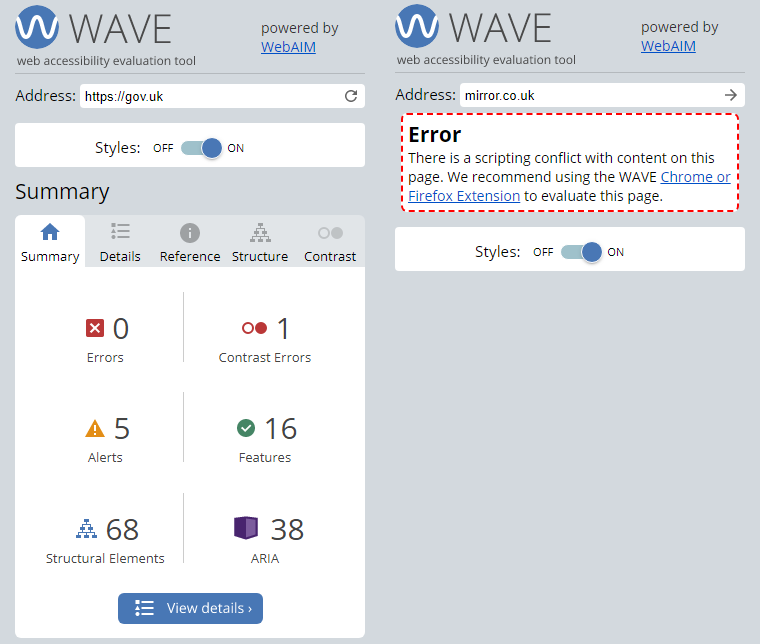
\includegraphics[keepaspectratio,width=\linewidth,height=\halfh]
{images/WAVE.png}

\caption[WAVE Overview]
{%
WAVE web tool header showing an overview for each test site.
}
\label{fig:WAVE}
\end{figure}



\section{Page Speed Insights aka. Lighthouse}

Page Speed Insights \parencite{PSIL} is a web tool based on the popular Lighthouse browser extension. Using the axe-core library as mentioned in Chapter \ref{tab:browser-extensions-info} this tool provides the same functionality as its browser extension counterpart. The tool can evaluate not only in consideration to accessibility but other metrics relevant to website quality. The web tool offers insight into basic performance, best practices, and Search Engine Optimization (SEO), in addition to assessing the accessibility of the tested website. After the accessibility audit is done the user may interact with the tool for further information on the found issues. These issues are represented in a list format, explaining what the current error is, as well as suggestions on how to fix said errors and examples of what they might look like. This list view can be seen in the given example in Figure~\ref{fig:PSIL}. Each of the elements in the list can be clicked on to view a more detailed version of the aforementioned errors and issues. 

\begin{figure}[tp]
\centering
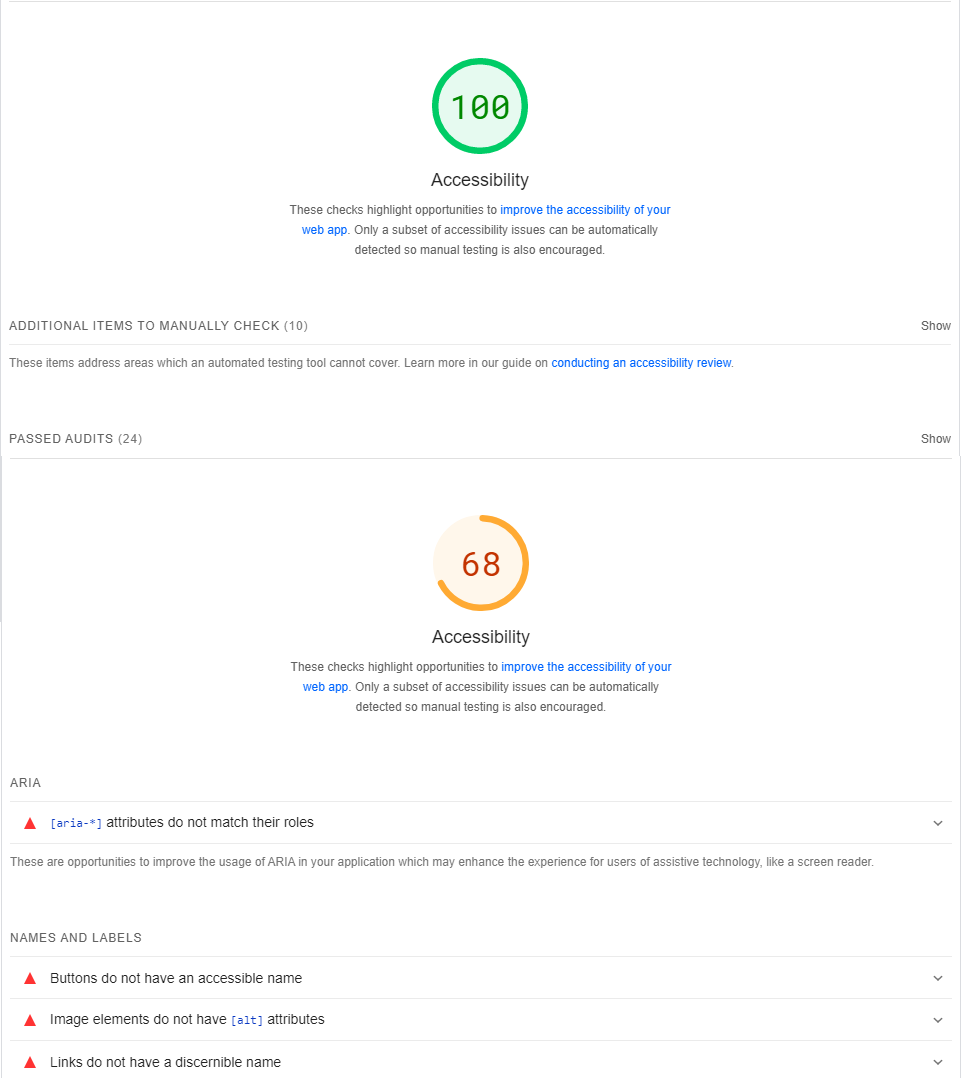
\includegraphics[keepaspectratio,width=\linewidth,height=\halfh]
{images/lighthouse.png}

\caption[Page Speed Insights Overview]
{%
Page Speed Insights (Lighthouse) web tool showing an overview for each test site.
}
\label{fig:PSIL}
\end{figure}




\section{Showcase videos}

In this survey, two websites were targeted for evaluation by the
aforementioned tools. For a good example concerning web accessibility,
the \url{https://www.gov.uk/} website was chosen whereas for the
negative example \url{https://www.mirror.co.uk/} was the choice. The
videos that were produced each showcase the interaction between the
user, the tools, and the website that is being evaluated
respectively. A video of this format was produced for Accessi
\parencite{Accessi_vid}, WAVE \parencite{WAVE_vid} and Page Speed
Insights (Lighthouse) \parencite{PageSpeedInsights_vid}. All of these
videos showcase the features of the tool that is being covered as well
as highlight a few extras the tool of each video might have over other
tools that might have a different focus. The outcome of all of the
videos is yet the same, as they all evaluate the positive example as
being very well rated and rating the negative example as being
non-compliant with the usual standards of accessibility for websites.



\section{Web Tools For Accessibility Audits Conclusion}

Concluding this chapter of the survey, its is fair to say that the
selection of web tools for accessibility audits is plentiful. There is
many tools which base themselves on the axe-core library and many
others which use their own librarys to assess the accessibility of a
website. As there is a standard in place which sets the boundarys for
accessibility usually all the tools come to the same general
conclusion for a given website, evaluating a good website as compliant
to accessibility and bad ones as being non-compliant. Through the big
selection of available tools it is adviseable to choose the one which
suits the needs of the auditor the most. An example would be when
maintaining a website on their own, the auditor might choose to use
either WAVE or Accessi, depending on if they prefer a list type of
view or the more interactive way. When looking for a more general
overview including other metrics like performance it is probably safe
to assume that Page Speed Insights will be more useful, as it always
includes a performance report as well as many other metrics
additionally to the accessibility assessment. The overall
recommendation is to first find a tool that is applicable to the
situation for each individual auditor. From this decision on the tools
commonly provide the same answer to a given test, where they focus on
different details depending on which tool was chosen.




\cleardoublepage

\chapter{Build Tools for Accessibility Audits}
\label{chap:Intro}

Accessibility can also be audited using tools that are integrated in the build
process.
Many of the browser extensions and web tools surveyed in this paper also offer
versions of the tools that can be used in the build process.
One benefit with these tools is that they offer instant feedback during development
without even opening the website, reducing the amount of work required for accessibility
auditing.
However, build tools for accessibility audits were not considered in this survey.


\cleardoublepage
% for now, switch to language english
% hack to force unix date for biblio, biblatex 3.11
\begin{otherlanguage}{english}
\printbibliography[heading=bibintoc]
\end{otherlanguage}


\end{document}

